%\includeonly{Introduction_thesis, The_Belle_Experiment, event_selection, cut_summary_table, continuum_suppression, branching_fraction_measurement, determination_of_signal_yield, gsim_and_toy_test, calibration, four_d_data_fit, bkgd_sub_mkpi, 4d_2d_toy, gsim_bias_correction, syst_wkst_wkpi, br_ul_sig, polarization, conclusion, bibliography}

%\includeonly{syst_wkst_wkpi, bibliography}


%%%%%%%%%%%%%%%%%%%%%%%%%%%%%%%%%%%%%%%%%%%%%%%%
%
%  PhD Thesis: master LATEX file 
%  -----------------------------
%
%%%%%%%%%%%%%%%%%%%%%%%%%%%%%%%%%%%%%%%%%%%%%%%%
%\documentclass[11pt,letter,twoside,psfig,epsfig,titlepage]{article}
\documentclass[11pt,letter,twoside,psfig,epsfig,]{article}
%\documentclass[11pt,a4paper,twoside,psfig,epsfig,titlepage]{report}
%\documentclass[11pt,a4paper,,psfig,epsfig, titlepage]{report}

\usepackage{a4wide}
\usepackage{graphicx}
\usepackage{amsmath}
\usepackage[square,numbers,sort&compress]{natbib}
\usepackage{url}
\usepackage{braket}
\usepackage[normal,small]{caption2}
\usepackage{afterpage}
\usepackage{float}
\usepackage{subfigure}
\usepackage{fancyheadings}
%\usepackage{doublespace}
\usepackage{xspace}
%\usepackage[mediumspace]{SIunits}
\usepackage{enumerate}
\usepackage{setspace}

\input epsf
\usepackage{tabularx}
\usepackage{epsfig}
\usepackage{verbatim}
\usepackage{subfigure}
\usepackage{geometry}                % See geometry.pdf to learn the layout options. There are lots.
\usepackage{graphicx}
\usepackage{amssymb}
%\usepackage{header}
\usepackage{epstopdf}
\usepackage{feynmf}
\usepackage{color}
\usepackage[section]{placeins}
%%%%%%%%%%%%%%%%%%%%%%%%%%%%%%%%%%%%%%%%%%%%%%%%%%%%%%%%%%%%%%%%%%%%%
%
%  CMS Common definitions style file
%
%  N.B. use of \newcommand rather than \newcommand means
%       that a definition is ignored if already specified
%
%                                              L. Taylor 18 Feb 2005
%%%%%%%%%%%%%%%%%%%%%%%%%%%%%%%%%%%%%%%%%%%%%%%%%%%%%%%%%%%%%%%%%%%%

% Some shorthand
% turn off italics
\newcommand {\etal}{\mbox{et al.}\xspace} %et al. - no preceding comma
\newcommand {\ie}{\mbox{i.e.}\xspace}     %i.e.
\newcommand {\eg}{\mbox{e.g.}\xspace}     %e.g.
\newcommand {\etc}{\mbox{etc.}\xspace}     %etc.
\newcommand {\vs}{\mbox{\sl vs.}\xspace}      %vs.
\newcommand {\mdash}{\ensuremath{\mathrm{-}}} % for use within formulas

% some terms whose definition we may change
\newcommand {\Lone}{Level-1\xspace} % Level-1 or L1 ?
\newcommand {\Ltwo}{Level-2\xspace}
\newcommand {\Lthree}{Level-3\xspace}

% Some software programs (alphabetized)
\newcommand{\ACERMC} {\textsc{AcerMC}\xspace}
\newcommand{\ALPGEN} {{\textsc{alpgen}}\xspace}
\newcommand{\CALCHEP} {{\textsc{CalcHEP}}\xspace}
\newcommand{\CHARYBDIS} {{\textsc{charybdis}}\xspace}
\newcommand{\CMKIN} {\textsc{cmkin}\xspace}
\newcommand{\CMSIM} {{\textsc{cmsim}}\xspace}
\newcommand{\CMSSW} {{\textsc{cmssw}}\xspace}
\newcommand{\COBRA} {{\textsc{cobra}}\xspace}
\newcommand{\COCOA} {{\textsc{cocoa}}\xspace}
\newcommand{\COMPHEP} {\textsc{CompHEP}\xspace}
\newcommand{\EVTGEN} {{\textsc{evtgen}}\xspace}
\newcommand{\FAMOS} {{\textsc{famos}}\xspace}
\newcommand{\GARCON} {\textsc{garcon}\xspace}
\newcommand{\GARFIELD} {{\textsc{garfield}}\xspace}
\newcommand{\GEANE} {{\textsc{geane}}\xspace}
\newcommand{\GEANTfour} {{\textsc{geant4}}\xspace}
\newcommand{\GEANTthree} {{\textsc{geant3}}\xspace}
\newcommand{\GEANT} {{\textsc{geant}}\xspace}
\newcommand{\HDECAY} {\textsc{hdecay}\xspace}
\newcommand{\HERWIG} {{\textsc{herwig}}\xspace}
\newcommand{\POWHEG} {{\textsc{powheg}}\xspace}
\newcommand{\HIGLU} {{\textsc{higlu}}\xspace}
\newcommand{\HIJING} {{\textsc{hijing}}\xspace}
\newcommand{\IGUANA} {\textsc{iguana}\xspace}
\newcommand{\ISAJET} {{\textsc{isajet}}\xspace}
\newcommand{\ISAPYTHIA} {{\textsc{isapythia}}\xspace}
\newcommand{\ISASUGRA} {{\textsc{isasugra}}\xspace}
\newcommand{\ISASUSY} {{\textsc{isasusy}}\xspace}
\newcommand{\ISAWIG} {{\textsc{isawig}}\xspace}
\newcommand{\MADGRAPH} {\textsc{MadGraph}\xspace}
\newcommand{\MCATNLO} {\textsc{mc@nlo}\xspace}
\newcommand{\MCFM} {\textsc{mcfm}\xspace}
\newcommand{\MILLEPEDE} {{\textsc{millepede}}\xspace}
\newcommand{\ORCA} {{\textsc{orca}}\xspace}
\newcommand{\OSCAR} {{\textsc{oscar}}\xspace}
\newcommand{\PHOTOS} {\textsc{photos}\xspace}
\newcommand{\PROSPINO} {\textsc{prospino}\xspace}
\newcommand{\PYTHIA} {{\textsc{pythia}}\xspace}
\newcommand{\SHERPA} {{\textsc{sherpa}}\xspace}
\newcommand{\TAUOLA} {\textsc{tauola}\xspace}
\newcommand{\TOPREX} {\textsc{TopReX}\xspace}
\newcommand{\XDAQ} {{\textsc{xdaq}}\xspace}


%  Experiments
\newcommand {\DZERO}{D0\xspace}     %etc.


% Measurements and units...

\newcommand{\de}{\ensuremath{^\circ}}
\newcommand{\ten}[1]{\ensuremath{\times \text{10}^\text{#1}}}
\newcommand{\unit}[1]{\ensuremath{\text{\,#1}}\xspace}
\newcommand{\mum}{\ensuremath{\,\mu\text{m}}\xspace}
\newcommand{\micron}{\ensuremath{\,\mu\text{m}}\xspace}
\newcommand{\cm}{\ensuremath{\,\text{cm}}\xspace}
\newcommand{\mm}{\ensuremath{\,\text{mm}}\xspace}
\newcommand{\mus}{\ensuremath{\,\mu\text{s}}\xspace}
\newcommand{\keV}{\ensuremath{\,\text{ke\hspace{-.08em}V}}\xspace}
\newcommand{\MeV}{\ensuremath{\,\text{Me\hspace{-.08em}V}}\xspace}
\newcommand{\GeV}{\ensuremath{\,\text{Ge\hspace{-.08em}V}}\xspace}
\newcommand{\GeVns}{\ensuremath{\text{Ge\hspace{-.08em}V}}\xspace}
\newcommand{\gev}{\GeV}
\newcommand{\TeV}{\ensuremath{\,\text{Te\hspace{-.08em}V}}\xspace}
\newcommand{\TeVns}{\ensuremath{\text{Te\hspace{-.08em}V}}\xspace}
\newcommand{\PeV}{\ensuremath{\,\text{Pe\hspace{-.08em}V}}\xspace}
\newcommand{\keVc}{\ensuremath{{\,\text{ke\hspace{-.08em}V\hspace{-0.16em}/\hspace{-0.08em}}c}}\xspace}
\newcommand{\MeVc}{\ensuremath{{\,\text{Me\hspace{-.08em}V\hspace{-0.16em}/\hspace{-0.08em}}c}}\xspace}
\newcommand{\GeVc}{\ensuremath{{\,\text{Ge\hspace{-.08em}V\hspace{-0.16em}/\hspace{-0.08em}}c}}\xspace}
\newcommand{\GeVcns}{\ensuremath{{\text{Ge\hspace{-.08em}V\hspace{-0.16em}/\hspace{-0.08em}}c}}\xspace}
\newcommand{\TeVc}{\ensuremath{{\,\text{Te\hspace{-.08em}V\hspace{-0.16em}/\hspace{-0.08em}}c}}\xspace}
\newcommand{\keVcc}{\ensuremath{{\,\text{ke\hspace{-.08em}V\hspace{-0.16em}/\hspace{-0.08em}}c^\text{2}}}\xspace}
\newcommand{\MeVcc}{\ensuremath{{\,\text{Me\hspace{-.08em}V\hspace{-0.16em}/\hspace{-0.08em}}c^\text{2}}}\xspace}
\newcommand{\GeVcc}{\ensuremath{{\,\text{Ge\hspace{-.08em}V\hspace{-0.16em}/\hspace{-0.08em}}c^\text{2}}}\xspace}
\newcommand{\TeVcc}{\ensuremath{{\,\text{Te\hspace{-.08em}V\hspace{-0.16em}/\hspace{-0.08em}}c^\text{2}}}\xspace}

\newcommand{\pbinv} {\mbox{\ensuremath{\,\text{pb}^\text{$-$1}}}\xspace}
\newcommand{\fbinv} {\mbox{\ensuremath{\,\text{fb}^\text{$-$1}}}\xspace}
\newcommand{\nbinv} {\mbox{\ensuremath{\,\text{nb}^\text{$-$1}}}\xspace}
\newcommand{\percms}{\ensuremath{\,\text{cm}^\text{$-$2}\,\text{s}^\text{$-$1}}\xspace}
\newcommand{\lumi}{\ensuremath{\mathcal{L}}\xspace}
\newcommand{\Lumi}{\ensuremath{\mathcal{L}}\xspace}%both upper and lower
%
% Need a convention here:
\newcommand{\LvLow}  {\ensuremath{\mathcal{L}=\text{10}^\text{32}\,\text{cm}^\text{$-$2}\,\text{s}^\text{$-$1}}\xspace}
\newcommand{\LLow}   {\ensuremath{\mathcal{L}=\text{10}^\text{33}\,\text{cm}^\text{$-$2}\,\text{s}^\text{$-$1}}\xspace}
\newcommand{\lowlumi}{\ensuremath{\mathcal{L}=\text{2}\times \text{10}^\text{33}\,\text{cm}^\text{$-$2}\,\text{s}^\text{$-$1}}\xspace}
\newcommand{\LMed}   {\ensuremath{\mathcal{L}=\text{2}\times \text{10}^\text{33}\,\text{cm}^\text{$-$2}\,\text{s}^\text{$-$1}}\xspace}
\newcommand{\LHigh}  {\ensuremath{\mathcal{L}=\text{10}^\text{34}\,\text{cm}^\text{$-$2}\,\text{s}^\text{$-$1}}\xspace}
\newcommand{\hilumi} {\ensuremath{\mathcal{L}=\text{10}^\text{34}\,\text{cm}^\text{$-$2}\,\text{s}^\text{$-$1}}\xspace}

% Physics symbols ...

\newcommand{\PT}{\ensuremath{p_{\mathrm{T}}}\xspace}
\newcommand{\pt}{\ensuremath{p_{\mathrm{T}}}\xspace}
\newcommand{\ET}{\ensuremath{E_{\mathrm{T}}}\xspace}
\newcommand{\HT}{\ensuremath{H_{\mathrm{T}}}\xspace}
\newcommand{\et}{\ensuremath{E_{\mathrm{T}}}\xspace}
\newcommand{\Em}{\ensuremath{E\hspace{-0.6em}/}\xspace}
\newcommand{\Pm}{\ensuremath{p\hspace{-0.5em}/}\xspace}
\newcommand{\PTm}{\ensuremath{{p}_\mathrm{T}\hspace{-1.02em}/}\xspace}
\newcommand{\PTslash}{\ensuremath{{p}_\mathrm{T}\hspace{-1.02em}/}\xspace}
\newcommand{\ETm}{\ensuremath{E_{\mathrm{T}}^{\text{miss}}}\xspace}
\newcommand{\MET}{\ETm}
\newcommand{\ETmiss}{\ETm}
\newcommand{\ETslash}{\ensuremath{E_{\mathrm{T}}\hspace{-1.1em}/\kern0.45em}\xspace}
\newcommand{\VEtmiss}{\ensuremath{{\vec E}_{\mathrm{T}}^{\text{miss}}}\xspace}

% roman face derivative
\newcommand{\dd}[2]{\ensuremath{\frac{\mathrm{d} #1}{\mathrm{d} #2}}}
\newcommand{\ddinline}[2]{\ensuremath{\mathrm{d} #1/\mathrm{d} #2}}
% absolute value
\newcommand{\abs}[1]{\ensuremath{\lvert #1 \rvert}}



\ifthenelse{\boolean{cms@italic}}{\newcommand{\cmsSymbolFace}{\relax}}{\newcommand{\cmsSymbolFace}{\mathrm}}

% Particle names which track the italic/non-italic face convention
\newcommand{\zp}{\ensuremath{\cmsSymbolFace{Z}^\prime}\xspace} % plain Z'
\newcommand{\JPsi}{\ensuremath{\cmsSymbolFace{J}\hspace{-.08em}/\hspace{-.14em}\psi}\xspace} % J/Psi (no mass)
\newcommand{\Z}{\ensuremath{\cmsSymbolFace{Z}}\xspace} % plain Z (no superscript 0)
\newcommand{\ttbar}{\ensuremath{\cmsSymbolFace{t}\overline{\cmsSymbolFace{t}}}\xspace} % t-tbar

% Extensions for missing names in PENNAMES % note no xspace, to match syntax in PENNAMES
\newcommand{\cPgn}{\ensuremath{\nu}} % generic neutrino
\providecommand{\Pgn}{\ensuremath{\nu}} % generic neutrino
\newcommand{\cPagn}{\ensuremath{\overline{\nu}}} % generic neutrino
\newcommand{\cPgg}{\ensuremath{\gamma}} % gamma
\newcommand{\cPJgy}{\ensuremath{\cmsSymbolFace{J}\hspace{-.08em}/\hspace{-.14em}\psi}} % J/Psi (no mass)
\newcommand{\cPZ}{\ensuremath{\cmsSymbolFace{Z}}} % plain Z (no superscript 0)
\newcommand{\cPZpr}{\ensuremath{\cmsSymbolFace{Z}^\prime}} % plain Z'
\newcommand{\cPqt}{\ensuremath{\cmsSymbolFace{t}}} % t for t quark
\newcommand{\cPqb}{\ensuremath{\cmsSymbolFace{b}}} % b for b quark
\newcommand{\cPqc}{\ensuremath{\cmsSymbolFace{c}}} % c for c quark
\newcommand{\cPqs}{\ensuremath{\cmsSymbolFace{s}}} % s for s quark
\newcommand{\cPqu}{\ensuremath{\cmsSymbolFace{u}}} % u for u quark
\newcommand{\cPqd}{\ensuremath{\cmsSymbolFace{d}}} % d for d quark
\newcommand{\cPq}{\ensuremath{\cmsSymbolFace{q}}} % generic quark
\newcommand{\cPg}{\ensuremath{\cmsSymbolFace{g}}} % generic gluon
\newcommand{\cPG}{\ensuremath{\cmsSymbolFace{G}}} % Graviton
\newcommand{\cPaqt}{\ensuremath{\overline{\cmsSymbolFace{t}}}} % t for t anti-quark
\newcommand{\cPaqb}{\ensuremath{\overline{\cmsSymbolFace{b}}}} % b for b anti-quark
\newcommand{\cPaqc}{\ensuremath{\overline{\cmsSymbolFace{c}}}} % c for c anti-quark
\newcommand{\cPaqs}{\ensuremath{\overline{\cmsSymbolFace{s}}}} % s for s anti-quark
\newcommand{\cPaqu}{\ensuremath{\overline{\cmsSymbolFace{u}}}} % u for u anti-quark
\newcommand{\cPaqd}{\ensuremath{\overline{\cmsSymbolFace{d}}}} % d for d anti-quark
\newcommand{\cPaq}{\ensuremath{\overline{\cmsSymbolFace{q}}}} % generic anti-quark
% future symbols from heppennames2
\providecommand{\PH}{\ensuremath{\cmsSymbolFace{H}}\xspace} % plain Higgs
\providecommand{\PJGy}{\ensuremath{\cmsSymbolFace{J}\hspace{-.08em}/\hspace{-.14em}\psi}\xspace} % J/Psi (no mass)
\providecommand{\PBzs}{\ensuremath{\cmsSymbolFace{B}^0_\cmsSymbolFace{s}}\xspace} % B^0_s
\providecommand{\Pg}{\ensuremath{\cmsSymbolFace{g}}} % generic gluon

% SM (still to be classified)

\newcommand{\AFB}{\ensuremath{A_\text{FB}}\xspace}
\newcommand{\wangle}{\ensuremath{\sin^{2}\theta_{\text{eff}}^\text{lept}(M^2_\Z)}\xspace}
\newcommand{\stat}{\ensuremath{\,\text{(stat.)}}\xspace}
\newcommand{\syst}{\ensuremath{\,\text{(syst.)}}\xspace}
\newcommand{\kt}{\ensuremath{k_{\mathrm{T}}}\xspace}

\newcommand{\BC}{\ensuremath{\cmsSymbolFace{B_{c}}}\xspace}
\newcommand{\bbarc}{\ensuremath{\cPqb\cPaqc}\xspace}
\newcommand{\bbbar}{\ensuremath{\cPqb\cPaqb}\xspace}
\newcommand{\ccbar}{\ensuremath{\cPqc\cPaqc}\xspace}
\newcommand{\bspsiphi}{\ensuremath{\cmsSymbolFace{B_s} \to \JPsi\, \phi}\xspace}
\newcommand{\EE}{\ensuremath{\Pep\Pem}\xspace}
\newcommand{\MM}{\ensuremath{\Pgmp\Pgmm}\xspace}
\newcommand{\TT}{\ensuremath{\Pgt^{+}\Pgt^{-}}\xspace}

%%%  E-gamma definitions
\newcommand{\HGG}{\ensuremath{\cmsSymbolFace{H}\to\gamma\gamma}}
\newcommand{\GAMJET}{\ensuremath{\gamma + \text{jet}}}
\newcommand{\PPTOJETS}{\ensuremath{\Pp\Pp\to\text{jets}}}
\newcommand{\PPTOGG}{\ensuremath{\Pp\Pp\to\gamma\gamma}}
\newcommand{\PPTOGAMJET}{\ensuremath{\Pp\Pp\to\gamma + \mathrm{jet}}}
\newcommand{\MH}{\ensuremath{M_{\mathrm{H}}}}
\newcommand{\RNINE}{\ensuremath{R_\mathrm{9}}}
\newcommand{\DR}{\ensuremath{\Delta R}}





%%%%%%
% From Albert
%

\newcommand{\ga}{\ensuremath{\gtrsim}}
\newcommand{\la}{\ensuremath{\lesssim}}
%
\newcommand{\swsq}{\ensuremath{\sin^2\theta_\cmsSymbolFace{W}}\xspace}
\newcommand{\cwsq}{\ensuremath{\cos^2\theta_\cmsSymbolFace{W}}\xspace}
\newcommand{\tanb}{\ensuremath{\tan\beta}\xspace}
\newcommand{\tanbsq}{\ensuremath{\tan^{2}\beta}\xspace}
\newcommand{\sidb}{\ensuremath{\sin 2\beta}\xspace}
\newcommand{\alpS}{\ensuremath{\alpha_S}\xspace}
\newcommand{\alpt}{\ensuremath{\tilde{\alpha}}\xspace}

\newcommand{\QL}{\ensuremath{\cmsSymbolFace{Q}_\cmsSymbolFace{L}}\xspace}
\newcommand{\sQ}{\ensuremath{\tilde{\cmsSymbolFace{Q}}}\xspace}
\newcommand{\sQL}{\ensuremath{\tilde{\cmsSymbolFace{Q}}_\cmsSymbolFace{L}}\xspace}
\newcommand{\ULC}{\ensuremath{\cmsSymbolFace{U}_\cmsSymbolFace{L}^\cmsSymbolFace{C}}\xspace}
\newcommand{\sUC}{\ensuremath{\tilde{\cmsSymbolFace{U}}^\cmsSymbolFace{C}}\xspace}
\newcommand{\sULC}{\ensuremath{\tilde{\cmsSymbolFace{U}}_\cmsSymbolFace{L}^\cmsSymbolFace{C}}\xspace}
\newcommand{\DLC}{\ensuremath{\cmsSymbolFace{D}_\cmsSymbolFace{L}^\cmsSymbolFace{C}}\xspace}
\newcommand{\sDC}{\ensuremath{\tilde{\cmsSymbolFace{D}}^\cmsSymbolFace{C}}\xspace}
\newcommand{\sDLC}{\ensuremath{\tilde{\cmsSymbolFace{D}}_\cmsSymbolFace{L}^\cmsSymbolFace{C}}\xspace}
\newcommand{\LL}{\ensuremath{\cmsSymbolFace{L}_\cmsSymbolFace{L}}\xspace}
\newcommand{\sL}{\ensuremath{\tilde{\cmsSymbolFace{L}}}\xspace}
\newcommand{\sLL}{\ensuremath{\tilde{\cmsSymbolFace{L}}_\cmsSymbolFace{L}}\xspace}
\newcommand{\ELC}{\ensuremath{\cmsSymbolFace{E}_\cmsSymbolFace{L}^\cmsSymbolFace{C}}\xspace}
\newcommand{\sEC}{\ensuremath{\tilde{\cmsSymbolFace{E}}^\cmsSymbolFace{C}}\xspace}
\newcommand{\sELC}{\ensuremath{\tilde{\cmsSymbolFace{E}}_\cmsSymbolFace{L}^\cmsSymbolFace{C}}\xspace}
\newcommand{\sEL}{\ensuremath{\tilde{\cmsSymbolFace{E}}_\cmsSymbolFace{L}}\xspace}
\newcommand{\sER}{\ensuremath{\tilde{\cmsSymbolFace{E}}_\cmsSymbolFace{R}}\xspace}
\newcommand{\sFer}{\ensuremath{\tilde{\cmsSymbolFace{f}}}\xspace}
\newcommand{\sQua}{\ensuremath{\tilde{\cmsSymbolFace{q}}}\xspace}
\newcommand{\sUp}{\ensuremath{\tilde{\cmsSymbolFace{u}}}\xspace}
\newcommand{\suL}{\ensuremath{\tilde{\cmsSymbolFace{u}}_\cmsSymbolFace{L}}\xspace}
\newcommand{\suR}{\ensuremath{\tilde{\cmsSymbolFace{u}}_\cmsSymbolFace{R}}\xspace}
\newcommand{\sDw}{\ensuremath{\tilde{\cmsSymbolFace{d}}}\xspace}
\newcommand{\sdL}{\ensuremath{\tilde{\cmsSymbolFace{d}}_\cmsSymbolFace{L}}\xspace}
\newcommand{\sdR}{\ensuremath{\tilde{\cmsSymbolFace{d}}_\cmsSymbolFace{R}}\xspace}
\newcommand{\sTop}{\ensuremath{\tilde{\cmsSymbolFace{t}}}\xspace}
\newcommand{\stL}{\ensuremath{\tilde{\cmsSymbolFace{t}}_\cmsSymbolFace{L}}\xspace}
\newcommand{\stR}{\ensuremath{\tilde{\cmsSymbolFace{t}}_\cmsSymbolFace{R}}\xspace}
\newcommand{\stone}{\ensuremath{\tilde{\cmsSymbolFace{t}}_1}\xspace}
\newcommand{\sttwo}{\ensuremath{\tilde{\cmsSymbolFace{t}}_2}\xspace}
\newcommand{\sBot}{\ensuremath{\tilde{\cmsSymbolFace{b}}}\xspace}
\newcommand{\sbL}{\ensuremath{\tilde{\cmsSymbolFace{b}}_\cmsSymbolFace{L}}\xspace}
\newcommand{\sbR}{\ensuremath{\tilde{\cmsSymbolFace{b}}_\cmsSymbolFace{R}}\xspace}
\newcommand{\sbone}{\ensuremath{\tilde{\cmsSymbolFace{b}}_1}\xspace}
\newcommand{\sbtwo}{\ensuremath{\tilde{\cmsSymbolFace{b}}_2}\xspace}
\newcommand{\sLep}{\ensuremath{\tilde{\cmsSymbolFace{l}}}\xspace}
\newcommand{\sLepC}{\ensuremath{\tilde{\cmsSymbolFace{l}}^\cmsSymbolFace{C}}\xspace}
\newcommand{\sEl}{\ensuremath{\tilde{\cmsSymbolFace{e}}}\xspace}
\newcommand{\sElC}{\ensuremath{\tilde{\cmsSymbolFace{e}}^\cmsSymbolFace{C}}\xspace}
\newcommand{\seL}{\ensuremath{\tilde{\cmsSymbolFace{e}}_\cmsSymbolFace{L}}\xspace}
\newcommand{\seR}{\ensuremath{\tilde{\cmsSymbolFace{e}}_\cmsSymbolFace{R}}\xspace}
\newcommand{\snL}{\ensuremath{\tilde{\nu}_L}\xspace}
\newcommand{\sMu}{\ensuremath{\tilde{\mu}}\xspace}
\newcommand{\sNu}{\ensuremath{\tilde{\nu}}\xspace}
\newcommand{\sTau}{\ensuremath{\tilde{\tau}}\xspace}
\newcommand{\Glu}{\ensuremath{\cmsSymbolFace{g}}\xspace}
\newcommand{\sGlu}{\ensuremath{\tilde{\cmsSymbolFace{g}}}\xspace}
\newcommand{\Wpm}{\ensuremath{\cmsSymbolFace{W}^{\pm}}\xspace}
\newcommand{\sWpm}{\ensuremath{\tilde{\cmsSymbolFace{W}}^{\pm}}\xspace}
\newcommand{\Wz}{\ensuremath{\cmsSymbolFace{W}^{0}}\xspace}
\newcommand{\sWz}{\ensuremath{\tilde{\cmsSymbolFace{W}}^{0}}\xspace}
\newcommand{\sWino}{\ensuremath{\tilde{\cmsSymbolFace{W}}}\xspace}
\newcommand{\Bz}{\ensuremath{\cmsSymbolFace{B}^{0}}\xspace}
\newcommand{\sBz}{\ensuremath{\tilde{\cmsSymbolFace{B}}^{0}}\xspace}
\newcommand{\sBino}{\ensuremath{\tilde{\cmsSymbolFace{B}}}\xspace}
\newcommand{\Zz}{\ensuremath{\cmsSymbolFace{Z}^{0}}\xspace}
\newcommand{\sZino}{\ensuremath{\tilde{\cmsSymbolFace{Z}}^{0}}\xspace}
\newcommand{\sGam}{\ensuremath{\tilde{\gamma}}\xspace}
\newcommand{\chiz}{\ensuremath{\tilde{\chi}^{0}}\xspace}
\newcommand{\chip}{\ensuremath{\tilde{\chi}^{+}}\xspace}
\newcommand{\chim}{\ensuremath{\tilde{\chi}^{-}}\xspace}
\newcommand{\chipm}{\ensuremath{\tilde{\chi}^{\pm}}\xspace}
\newcommand{\Hone}{\ensuremath{\cmsSymbolFace{H}_\cmsSymbolFace{d}}\xspace}
\newcommand{\sHone}{\ensuremath{\tilde{\cmsSymbolFace{H}}_\cmsSymbolFace{d}}\xspace}
\newcommand{\Htwo}{\ensuremath{\cmsSymbolFace{H}_\cmsSymbolFace{u}}\xspace}
\newcommand{\sHtwo}{\ensuremath{\tilde{\cmsSymbolFace{H}}_\cmsSymbolFace{u}}\xspace}
\newcommand{\sHig}{\ensuremath{\tilde{\cmsSymbolFace{H}}}\xspace}
\newcommand{\sHa}{\ensuremath{\tilde{\cmsSymbolFace{H}}_\cmsSymbolFace{a}}\xspace}
\newcommand{\sHb}{\ensuremath{\tilde{\cmsSymbolFace{H}}_\cmsSymbolFace{b}}\xspace}
\newcommand{\sHpm}{\ensuremath{\tilde{\cmsSymbolFace{H}}^{\pm}}\xspace}
\newcommand{\hz}{\ensuremath{\cmsSymbolFace{h}^{0}}\xspace}
\newcommand{\Hz}{\ensuremath{\cmsSymbolFace{H}^{0}}\xspace}
\newcommand{\Az}{\ensuremath{\cmsSymbolFace{A}^{0}}\xspace}
\newcommand{\Hpm}{\ensuremath{\cmsSymbolFace{H}^{\pm}}\xspace}
\newcommand{\sGra}{\ensuremath{\tilde{\cmsSymbolFace{G}}}\xspace}
%
\newcommand{\mtil}{\ensuremath{\tilde{m}}\xspace}
%
\newcommand{\rpv}{\ensuremath{\rlap{\kern.2em/}R}\xspace}
\newcommand{\LLE}{\ensuremath{LL\bar{E}}\xspace}
\newcommand{\LQD}{\ensuremath{LQ\bar{D}}\xspace}
\newcommand{\UDD}{\ensuremath{\overline{UDD}}\xspace}
\newcommand{\Lam}{\ensuremath{\lambda}\xspace}
\newcommand{\Lamp}{\ensuremath{\lambda'}\xspace}
\newcommand{\Lampp}{\ensuremath{\lambda''}\xspace}
%
\newcommand{\spinbd}[2]{\ensuremath{\bar{#1}_{\dot{#2}}}\xspace}

\newcommand{\MD}{\ensuremath{{M_\mathrm{D}}}\xspace}% ED mass
\newcommand{\Mpl}{\ensuremath{{M_\mathrm{Pl}}}\xspace}% Planck mass
\newcommand{\Rinv} {\ensuremath{{R}^{-1}}\xspace}
\endinput 
\newcommand\rs{\raisebox{1.0ex}[-1.0ex]}
\newcommand{\ra}{\ensuremath{\rightarrow}}
\newcommand{\znunu}{\ensuremath{{\text Z} \ra \nu\bar{\nu}}\xspace}
\newcommand{\zmumu}{\ensuremath{{\text Z} \ra \mu\mu}\xspace}
\newcommand{\dyllFifty}{\ensuremath{{\text Z/\gamma^{*}} \ra l^{+}l^{-}(m_{ll}>50)}\xspace}
\newcommand{\dyllTen}{\ensuremath{{\text Z/\gamma^{*}} \ra l^{+}l^{-}(10<m_{ll}<50)}\xspace}
\newcommand{\dyll}{\ensuremath{{\text Z/\gamma^{*}} \ra l^{+}l^{-}}\xspace}
\newcommand{\wmunu}{\ensuremath{{\text W} \ra \mu\nu}}
\newcommand{\wlnu}{\ensuremath{{\text W}\!\ra\!l\nu}\xspace}
\newcommand{\wtaunu}{\ensuremath{{\text W} \ra \tau\nu}}
\newcommand{\dphi}{\ensuremath{\Delta \phi}}
\newcommand{\dphijj}{\ensuremath{\Delta \phi_{ j1,j2}}}
\newcommand{\Pt}{\ensuremath{{p_{\text T}}}\xspace}
\newcommand{\pts}{\ensuremath{p_{\text T}{\text s}}\xspace}
\newcommand{\Et}{\ensuremath{{E_{\text T}}}\xspace}
\newcommand{\ptjf}{\ensuremath{p_{\rm T}^{ {\rm j}_1} }}
\newcommand{\ptjs}{\ensuremath{p_{\rm T}^{ {\rm j}_2} }}
\newcommand{\ptjt}{\ensuremath{p_{\rm T}^{ {\rm j}_3} }}
\newcommand{\etajf}{\ensuremath{\eta^{ {\rm j}_1} }}
\newcommand{\etajs}{\ensuremath{\eta^{ {\rm j}_2} }}
\newcommand{\etajt}{\ensuremath{\eta^{ {\rm j}_3} }}
\newcommand{\ttj}{\ensuremath{\rm{t}\bar{\rm{t}} + jets}\xspace}
\newcommand{\ttc}{\ensuremath{\rm{t}\;\;(\text {t-channel})}\xspace}
\newcommand{\tsc}{\ensuremath{\rm{t}\;\;(\text {s-channel})}\xspace}
\newcommand{\ttwc}{\ensuremath{\rm{t}\;\;(\text {tW-channel})}\xspace}
\newcommand{\tbtc}{\ensuremath{\bar{\rm{t}}\;\;(\text {t-channel})}\xspace}
\newcommand{\tbsc}{\ensuremath{\bar{\rm{t}}\;\;(\text {s-channel})}\xspace}
\newcommand{\tbtwc}{\ensuremath{\bar{\rm{t}}\;\;(\text {tW-channel})}\xspace}

\newcommand{\wj}{\ensuremath{\rm W + jets}\xspace}
\newcommand{\zj}{\ensuremath{\rm Z + jets}\xspace}

\newcommand{\al}{\ensuremath{\alpha}}
\newcommand{\alt}{\ensuremath{\alpha_{\text{T}}}\xspace}
\newcommand{\etaabs}{\ensuremath{|\eta|}}
%\newcommand{\gev}{\ensuremath{\mathrm{\,Ge\kern -0.1em V}}}
\newcommand{\pb}{\ensuremath{pb^{-1}}}
\newcommand{\mjj}{\ensuremath{M_{\text{inv}}^{j1,j2}}}
%\newcommand{\ttbar}{\ensuremath{t\bar{t}}}
\newcommand{\chiznew}{\ensuremath{\chi^{0}}\xspace}
\newcommand{\chipnew}{\ensuremath{\chi^{+}}\xspace}
\newcommand{\sQuanew}{\ensuremath{\tilde{\rm q}}\xspace}
\newcommand{\sGlunew}{\ensuremath{\tilde{\rm g}}\xspace}
\newcommand{\ttNew}{\ensuremath{\rm{t}\bar{\rm{t}}}\xspace}
\newcommand{\tev}{\TeV}
%<TW date="30/10/2010">
%\newcommand{\Et}{E_{T}}
\newcommand{\combIso}{Iso_{\textrm{comb.}}}
\renewcommand{\arraystretch}{1.2}
\newcommand{\bigNum}[2]{#1 \, \times \, 10 \, ^{#2}}
%</TW>

\newcommand{\raT}{\ensuremath{R_{\alt}}}
\newcommand{\RaT}{\ensuremath{R_{\alt}}\xspace}

\newcommand{\Ttwocc}{\ensuremath{\text{pp}\,\ra\,\sTop\sTop^{*}\,\ra\,\text{c}\chiz\,\bar{\text{c}}\chiz}}
\newcommand{\Ttwott}{\ensuremath{\text{pp}\,\ra\,\sTop\sTop^{*}\,\ra\,\text{t}\chiz\,\bar{\text{t}}\chiz}}
\newcommand{\Ttwodegen}{\ensuremath{\text{pp}\,\ra\,\sTop\sTop^{*}\,\ra\,\text{b}\chiz W\,\text{b}\chiz W}}

\newcommand\T{\rule{0pt}{2.6ex}}
\newcommand\B{\rule[-1.2ex]{0pt}{0pt}}

\def\eslash{{\hbox{$E$\kern-0.6em\lower-.05ex\hbox{/}\kern0.10em}}}
\def\vecmet{\mbox{$\vec{\eslash}_T$}} %missing ET vector
\def\vecet{\mbox{$\vec{E}_\text{T}$}} % ET vector
\def\MET{\mbox{$\eslash_\text{T}$}\xspace}
\def\met{\mbox{$\eslash_\text{T}$}\xspace}
\def\pfmet{\mbox{$\eslash_\text{T}^{\rm PF}$}\xspace}
\def\mex{\mbox{$\eslash_\text{x}$}} %missing Ex
\def\mey{\mbox{$\eslash_\text{y}$}} %missing Ey
\def\mepar{\mbox{$\eslash_\parallel$}}
\def\meperp{\mbox{$\eslash_\perp$}}
\def\Zmm{Z \rightarrow \mu\mu}
\def\metvec{\mbox{$\vec{\met}$}\xspace}
\def\metvecrec{\mbox{$\vec{\met}^{\rm rec}$}\xspace}
\def\metvecgen{\mbox{$\vec{\met}^{\rm gen}$}\xspace}
\def\metgen{\mbox{$\met^{\rm gen}$}\xspace}
\def\metparl{\mbox{$\mepar^{\rm rec}$}\xspace}
\def\metperp{\mbox{$\meperp^{\rm rec}$}\xspace}
\def\deltamet{\mbox{$\Delta\met$}\xspace}
\def\pthat{\mbox{$\hat{p}_T$}\xspace}
\def\hslash{{\hbox{$H$\kern-0.8em\lower-.05ex\hbox{/}\kern0.10em}}}
\def\MHT{\mbox{$\hslash_\text{T}$}\xspace}
\def\mht{\mbox{$\hslash_\text{T}$}\xspace}
\def\mhtmet{\mbox{$\hslash_\text{T} / \eslash_\text{T}$}\xspace}
\def\mhtmetmiss{\mbox{$\H_\text{T}^{\rm miss} / \E_\text{T}^{\rm miss}$}\xspace}
\def\rmhtmet{\mbox{$R_{\hslash_\text{T} / \eslash_\text{T}}$}\xspace}
\def\sumet{\mbox{$\sum \rm{E}_\text{T}$}\xspace}
\def\scalht{\mbox{$H_\text{T}$}\xspace}
\def\etmiss{\mbox{$\eslash_\text{T}$}\xspace}
\def\htmiss{\mbox{$\hslash_\text{T}$}\xspace}
\def\mtt{\mbox{$\rm{M}_\text{T2}$}\xspace}
\def\rmec{\mbox{$R_{\mht/\met}$}\xspace}
\def\bdphi{\mbox{$\Delta\phi^{*}$}\xspace}
\def\bigeslash{{\hbox{$E$\kern-0.38em\lower-.05ex\hbox{/}\kern0.10em}}}
\def\bigmet{\mbox{$\bigeslash_T$}}
\def\bighslash{{\hbox{$H$\kern-0.6em\lower-.05ex\hbox{/}\kern0.10em}}}
\def\bigmht{\mbox{$\bighslash_T$}}
\def\incl{\includegraphics[width=0.49\linewidth]}
\def\inclrot{\includegraphics[angle=90,width=0.47\linewidth]}
\def\INCL{\includegraphics[angle=90,width=0.45\linewidth]}
\def\Incl{\includegraphics[angle=90,width=0.60\linewidth]}
\def\cls{\mbox{CL$_s$}\xspace}

\newcommand{\zero}{\ensuremath{\phantom{0}}}

\newcommand{\kfactor}{\ensuremath{k\text{-factor}}\xspace}
\newcommand{\kfactors}{\ensuremath{k\text{-factors}}\xspace}
\newcommand{\njet}{\ensuremath{n_{\text{jet}}}\xspace}
\newcommand{\njetlow}{\ensuremath{2 \leq \njet \leq 3}\xspace}
\newcommand{\njethigh}{\ensuremath{\njet \geq 4}\xspace}
\newcommand{\nb}{\ensuremath{n_{\text{b}}}\xspace}
\newcommand{\alphat}{\ensuremath{\alpha_{\text{T}}}\xspace}
\newcommand{\alphatcut}{\ensuremath{\alpha_{\text{T}}^{\text{cut}}}\xspace}
\newcommand{\htalphat}{\texttt{HT\_AlphaT}\xspace}
\newcommand{\photon}{\texttt{Photon}\xspace}
\newcommand{\muht}{\texttt{Mu\_HT}\xspace}
\newcommand{\httrigger}{\texttt{HT}\xspace}
\newcommand{\mt}{\ensuremath{M_{\textrm T}}\xspace}
\newcommand{\gj}{\ensuremath{\gamma} + jets\xspace}
\newcommand{\mj}{\ensuremath{\mu} + jets\xspace}
\newcommand{\mmj}{\ensuremath{\mu\mu} + jets\xspace}
\newcommand{\npre}{\ensuremath{N_{\textrm{pred}}}\xspace}
\newcommand{\nobs}{\ensuremath{N_{\textrm{obs}}}\xspace}
\newcommand{\njets}{\ensuremath{N_{\textrm{jet}}}\xspace}
\newcommand{\sq}{\ensuremath{\tilde{\rm q}}\xspace}
\newcommand{\st}{\ensuremath{\tilde{\rm t}}\xspace}
\newcommand{\gl}{\ensuremath{\tilde{\rm g}}\xspace}
\newcommand{\dht}{\ensuremath{\Delta\scalht}\xspace}
\newcommand{\ewk}{\ensuremath{\mathrm{EWK}}\xspace}
\newcommand{\qcd}{\ensuremath{\mathrm{QCD}}\xspace}
\newcommand{\fZinv}[1]{\ensuremath{f_{\rm Zinv}^{#1}}\xspace}
\newcommand{\zInv}[1]{\ensuremath{Z_{\rm inv}^{#1}}\xspace}
\newcommand{\meanHt}[1]{\ensuremath{\langle \HT \rangle^{#1}}\xspace}
\newcommand{\lk}[2]{\ensuremath{L^{\rm #1}_{\rm #2}}\xspace}
\newcommand{\sep}{\ensuremath{68^{\mathrm{th}}}\xspace}
\newcommand{\partonht}{\ensuremath{\scalht^{\rm parton}}\xspace}
\newcommand{\nparton}{\ensuremath{N^{\rm parton}}\xspace}
\providecommand{\e}[1]{\ensuremath{\times 10^{#1}}}

% Some shorthand
% turn off italics
\newcommand {\etal}{\mbox{et al.}\xspace} %et al. - no preceding comma
\newcommand {\ie}{\mbox{i.e.}\xspace}     %i.e.
\newcommand {\eg}{\mbox{e.g.}\xspace}     %e.g.
\newcommand {\etc}{\mbox{etc.}\xspace}     %etc.
\newcommand {\vs}{\mbox{\sl vs.}\xspace}      %vs.
\newcommand {\mdash}{\ensuremath{\mathrm{-}}} % for use within formulas

% some terms whose definition we may change
\newcommand {\Lone}{Level-1\xspace} % Level-1 or L1 ?
\newcommand {\Ltwo}{Level-2\xspace}
\newcommand {\Lthree}{Level-3\xspace}

% Some software programs (alphabetized)
\newcommand{\ACERMC} {\textsc{AcerMC}\xspace}
\newcommand{\ALPGEN} {{\textsc{alpgen}}\xspace}
\newcommand{\CALCHEP} {{\textsc{CalcHEP}}\xspace}
\newcommand{\CHARYBDIS} {{\textsc{charybdis}}\xspace}
\newcommand{\CMKIN} {\textsc{cmkin}\xspace}
\newcommand{\CMSIM} {{\textsc{cmsim}}\xspace}
\newcommand{\CMSSW} {{\textsc{cmssw}}\xspace}
\newcommand{\COBRA} {{\textsc{cobra}}\xspace}
\newcommand{\COCOA} {{\textsc{cocoa}}\xspace}
\newcommand{\COMPHEP} {\textsc{CompHEP}\xspace}
\newcommand{\EVTGEN} {{\textsc{evtgen}}\xspace}
\newcommand{\FAMOS} {{\textsc{famos}}\xspace}
\newcommand{\GARCON} {\textsc{garcon}\xspace}
\newcommand{\GARFIELD} {{\textsc{garfield}}\xspace}
\newcommand{\GEANE} {{\textsc{geane}}\xspace}
\newcommand{\GEANTfour} {{\textsc{geant4}}\xspace}
\newcommand{\GEANTthree} {{\textsc{geant3}}\xspace}
\newcommand{\GEANT} {{\textsc{geant}}\xspace}
\newcommand{\HDECAY} {\textsc{hdecay}\xspace}
\newcommand{\HERWIG} {{\textsc{herwig}}\xspace}
\newcommand{\POWHEG} {{\textsc{powheg}}\xspace}
\newcommand{\HIGLU} {{\textsc{higlu}}\xspace}
\newcommand{\HIJING} {{\textsc{hijing}}\xspace}
\newcommand{\IGUANA} {\textsc{iguana}\xspace}
\newcommand{\ISAJET} {{\textsc{isajet}}\xspace}
\newcommand{\ISAPYTHIA} {{\textsc{isapythia}}\xspace}
\newcommand{\ISASUGRA} {{\textsc{isasugra}}\xspace}
\newcommand{\ISASUSY} {{\textsc{isasusy}}\xspace}
\newcommand{\ISAWIG} {{\textsc{isawig}}\xspace}
\newcommand{\MADGRAPH} {\textsc{MadGraph}\xspace}
\newcommand{\MCATNLO} {\textsc{mc@nlo}\xspace}
\newcommand{\MCFM} {\textsc{mcfm}\xspace}
\newcommand{\MILLEPEDE} {{\textsc{millepede}}\xspace}
\newcommand{\ORCA} {{\textsc{orca}}\xspace}
\newcommand{\OSCAR} {{\textsc{oscar}}\xspace}
\newcommand{\PHOTOS} {\textsc{photos}\xspace}
\newcommand{\PROSPINO} {\textsc{prospino}\xspace}
\newcommand{\PYTHIA} {{\textsc{pythia}}\xspace}
\newcommand{\SHERPA} {{\textsc{sherpa}}\xspace}
\newcommand{\TAUOLA} {\textsc{tauola}\xspace}
\newcommand{\TOPREX} {\textsc{TopReX}\xspace}
\newcommand{\XDAQ} {{\textsc{xdaq}}\xspace}


%  Experiments
\newcommand {\DZERO}{D0\xspace}     %etc.


% Measurements and units...

\newcommand{\de}{\ensuremath{^\circ}}
\newcommand{\ten}[1]{\ensuremath{\times \text{10}^\text{#1}}}
\newcommand{\unit}[1]{\ensuremath{\text{\,#1}}\xspace}
\newcommand{\mum}{\ensuremath{\,\mu\text{m}}\xspace}
\newcommand{\micron}{\ensuremath{\,\mu\text{m}}\xspace}
\newcommand{\cm}{\ensuremath{\,\text{cm}}\xspace}
\newcommand{\mm}{\ensuremath{\,\text{mm}}\xspace}
\newcommand{\mus}{\ensuremath{\,\mu\text{s}}\xspace}
\newcommand{\keV}{\ensuremath{\,\text{ke\hspace{-.08em}V}}\xspace}
\newcommand{\MeV}{\ensuremath{\,\text{Me\hspace{-.08em}V}}\xspace}
\newcommand{\GeV}{\ensuremath{\,\text{Ge\hspace{-.08em}V}}\xspace}
\newcommand{\GeVns}{\ensuremath{\text{Ge\hspace{-.08em}V}}\xspace}
\newcommand{\gev}{\GeV}
\newcommand{\TeV}{\ensuremath{\,\text{Te\hspace{-.08em}V}}\xspace}
\newcommand{\TeVns}{\ensuremath{\text{Te\hspace{-.08em}V}}\xspace}
\newcommand{\PeV}{\ensuremath{\,\text{Pe\hspace{-.08em}V}}\xspace}
\newcommand{\keVc}{\ensuremath{{\,\text{ke\hspace{-.08em}V\hspace{-0.16em}/\hspace{-0.08em}}c}}\xspace}
\newcommand{\MeVc}{\ensuremath{{\,\text{Me\hspace{-.08em}V\hspace{-0.16em}/\hspace{-0.08em}}c}}\xspace}
\newcommand{\GeVc}{\ensuremath{{\,\text{Ge\hspace{-.08em}V\hspace{-0.16em}/\hspace{-0.08em}}c}}\xspace}
\newcommand{\GeVcns}{\ensuremath{{\text{Ge\hspace{-.08em}V\hspace{-0.16em}/\hspace{-0.08em}}c}}\xspace}
\newcommand{\TeVc}{\ensuremath{{\,\text{Te\hspace{-.08em}V\hspace{-0.16em}/\hspace{-0.08em}}c}}\xspace}
\newcommand{\keVcc}{\ensuremath{{\,\text{ke\hspace{-.08em}V\hspace{-0.16em}/\hspace{-0.08em}}c^\text{2}}}\xspace}
\newcommand{\MeVcc}{\ensuremath{{\,\text{Me\hspace{-.08em}V\hspace{-0.16em}/\hspace{-0.08em}}c^\text{2}}}\xspace}
\newcommand{\GeVcc}{\ensuremath{{\,\text{Ge\hspace{-.08em}V\hspace{-0.16em}/\hspace{-0.08em}}c^\text{2}}}\xspace}
\newcommand{\TeVcc}{\ensuremath{{\,\text{Te\hspace{-.08em}V\hspace{-0.16em}/\hspace{-0.08em}}c^\text{2}}}\xspace}

\newcommand{\pbinv} {\mbox{\ensuremath{\,\text{pb}^\text{$-$1}}}\xspace}
\newcommand{\fbinv} {\mbox{\ensuremath{\,\text{fb}^\text{$-$1}}}\xspace}
\newcommand{\nbinv} {\mbox{\ensuremath{\,\text{nb}^\text{$-$1}}}\xspace}
\newcommand{\percms}{\ensuremath{\,\text{cm}^\text{$-$2}\,\text{s}^\text{$-$1}}\xspace}
\newcommand{\lumi}{\ensuremath{\mathcal{L}}\xspace}
\newcommand{\Lumi}{\ensuremath{\mathcal{L}}\xspace}%both upper and lower
%
% Need a convention here:
\newcommand{\LvLow}  {\ensuremath{\mathcal{L}=\text{10}^\text{32}\,\text{cm}^\text{$-$2}\,\text{s}^\text{$-$1}}\xspace}
\newcommand{\LLow}   {\ensuremath{\mathcal{L}=\text{10}^\text{33}\,\text{cm}^\text{$-$2}\,\text{s}^\text{$-$1}}\xspace}
\newcommand{\lowlumi}{\ensuremath{\mathcal{L}=\text{2}\times \text{10}^\text{33}\,\text{cm}^\text{$-$2}\,\text{s}^\text{$-$1}}\xspace}
\newcommand{\LMed}   {\ensuremath{\mathcal{L}=\text{2}\times \text{10}^\text{33}\,\text{cm}^\text{$-$2}\,\text{s}^\text{$-$1}}\xspace}
\newcommand{\LHigh}  {\ensuremath{\mathcal{L}=\text{10}^\text{34}\,\text{cm}^\text{$-$2}\,\text{s}^\text{$-$1}}\xspace}
\newcommand{\hilumi} {\ensuremath{\mathcal{L}=\text{10}^\text{34}\,\text{cm}^\text{$-$2}\,\text{s}^\text{$-$1}}\xspace}

% Physics symbols ...

\newcommand{\PT}{\ensuremath{p_{\mathrm{T}}}\xspace}
\newcommand{\pt}{\ensuremath{p_{\mathrm{T}}}\xspace}
\newcommand{\ET}{\ensuremath{E_{\mathrm{T}}}\xspace}
\newcommand{\HT}{\ensuremath{H_{\mathrm{T}}}\xspace}
\newcommand{\et}{\ensuremath{E_{\mathrm{T}}}\xspace}
\newcommand{\Em}{\ensuremath{E\hspace{-0.6em}/}\xspace}
\newcommand{\Pm}{\ensuremath{p\hspace{-0.5em}/}\xspace}
\newcommand{\PTm}{\ensuremath{{p}_\mathrm{T}\hspace{-1.02em}/}\xspace}
\newcommand{\PTslash}{\ensuremath{{p}_\mathrm{T}\hspace{-1.02em}/}\xspace}
\newcommand{\ETm}{\ensuremath{E_{\mathrm{T}}^{\text{miss}}}\xspace}
%\newcommand{\MET}{\ETm}
%\newcommand{\ETmiss}{\ETm}
\newcommand{\ETslash}{\ensuremath{E_{\mathrm{T}}\hspace{-1.1em}/\kern0.45em}\xspace}
\newcommand{\VEtmiss}{\ensuremath{{\vec E}_{\mathrm{T}}^{\text{miss}}}\xspace}

% roman face derivative
\newcommand{\dd}[2]{\ensuremath{\frac{\mathrm{d} #1}{\mathrm{d} #2}}}
\newcommand{\ddinline}[2]{\ensuremath{\mathrm{d} #1/\mathrm{d} #2}}
% absolute value
\newcommand{\abs}[1]{\ensuremath{\lvert #1 \rvert}}


\newcommand{\cmsSymbolFace}{\relax}
% Particle names which track the italic/non-italic face convention
\newcommand{\zp}{\ensuremath{\cmsSymbolFace{Z}^\prime}\xspace} % plain Z'
\newcommand{\JPsi}{\ensuremath{\cmsSymbolFace{J}\hspace{-.08em}/\hspace{-.14em}\psi}\xspace} % J/Psi (no mass)
\newcommand{\Z}{\ensuremath{\cmsSymbolFace{Z}}\xspace} % plain Z (no superscript 0)
\newcommand{\ttbar}{\ensuremath{\cmsSymbolFace{t}\overline{\cmsSymbolFace{t}}}\xspace} % t-tbar

% Extensions for missing names in PENNAMES % note no xspace, to match syntax in PENNAMES
\newcommand{\cPgn}{\ensuremath{\nu}} % generic neutrino
\providecommand{\Pgn}{\ensuremath{\nu}} % generic neutrino
\newcommand{\cPagn}{\ensuremath{\overline{\nu}}} % generic neutrino
\newcommand{\cPgg}{\ensuremath{\gamma}} % gamma
\newcommand{\cPJgy}{\ensuremath{\cmsSymbolFace{J}\hspace{-.08em}/\hspace{-.14em}\psi}} % J/Psi (no mass)
\newcommand{\cPZ}{\ensuremath{\cmsSymbolFace{Z}}} % plain Z (no superscript 0)
\newcommand{\cPZpr}{\ensuremath{\cmsSymbolFace{Z}^\prime}} % plain Z'
\newcommand{\cPqt}{\ensuremath{\cmsSymbolFace{t}}} % t for t quark
\newcommand{\cPqb}{\ensuremath{\cmsSymbolFace{b}}} % b for b quark
\newcommand{\cPqc}{\ensuremath{\cmsSymbolFace{c}}} % c for c quark
\newcommand{\cPqs}{\ensuremath{\cmsSymbolFace{s}}} % s for s quark
\newcommand{\cPqu}{\ensuremath{\cmsSymbolFace{u}}} % u for u quark
\newcommand{\cPqd}{\ensuremath{\cmsSymbolFace{d}}} % d for d quark
\newcommand{\cPq}{\ensuremath{\cmsSymbolFace{q}}} % generic quark
\newcommand{\cPg}{\ensuremath{\cmsSymbolFace{g}}} % generic gluon
\newcommand{\cPG}{\ensuremath{\cmsSymbolFace{G}}} % Graviton
\newcommand{\cPaqt}{\ensuremath{\overline{\cmsSymbolFace{t}}}} % t for t anti-quark
\newcommand{\cPaqb}{\ensuremath{\overline{\cmsSymbolFace{b}}}} % b for b anti-quark
\newcommand{\cPaqc}{\ensuremath{\overline{\cmsSymbolFace{c}}}} % c for c anti-quark
\newcommand{\cPaqs}{\ensuremath{\overline{\cmsSymbolFace{s}}}} % s for s anti-quark
\newcommand{\cPaqu}{\ensuremath{\overline{\cmsSymbolFace{u}}}} % u for u anti-quark
\newcommand{\cPaqd}{\ensuremath{\overline{\cmsSymbolFace{d}}}} % d for d anti-quark
\newcommand{\cPaq}{\ensuremath{\overline{\cmsSymbolFace{q}}}} % generic anti-quark
% future symbols from heppennames2
\providecommand{\PH}{\ensuremath{\cmsSymbolFace{H}}\xspace} % plain Higgs
\providecommand{\PJGy}{\ensuremath{\cmsSymbolFace{J}\hspace{-.08em}/\hspace{-.14em}\psi}\xspace} % J/Psi (no mass)
\providecommand{\PBzs}{\ensuremath{\cmsSymbolFace{B}^0_\cmsSymbolFace{s}}\xspace} % B^0_s
\providecommand{\Pg}{\ensuremath{\cmsSymbolFace{g}}} % generic gluon

% SM (still to be classified)

\newcommand{\AFB}{\ensuremath{A_\text{FB}}\xspace}
\newcommand{\wangle}{\ensuremath{\sin^{2}\theta_{\text{eff}}^\text{lept}(M^2_\Z)}\xspace}
\newcommand{\stat}{\ensuremath{\,\text{(stat.)}}\xspace}
\newcommand{\syst}{\ensuremath{\,\text{(syst.)}}\xspace}
\newcommand{\kt}{\ensuremath{k_{\mathrm{T}}}\xspace}

\newcommand{\BC}{\ensuremath{\cmsSymbolFace{B_{c}}}\xspace}
\newcommand{\bbarc}{\ensuremath{\cPqb\cPaqc}\xspace}
\newcommand{\bbbar}{\ensuremath{\cPqb\cPaqb}\xspace}
\newcommand{\ccbar}{\ensuremath{\cPqc\cPaqc}\xspace}
\newcommand{\bspsiphi}{\ensuremath{\cmsSymbolFace{B_s} \to \JPsi\, \phi}\xspace}
\newcommand{\EE}{\ensuremath{\Pep\Pem}\xspace}
\newcommand{\MM}{\ensuremath{\Pgmp\Pgmm}\xspace}
\newcommand{\TT}{\ensuremath{\Pgt^{+}\Pgt^{-}}\xspace}

%%%  E-gamma definitions
\newcommand{\HGG}{\ensuremath{\cmsSymbolFace{H}\to\gamma\gamma}}
\newcommand{\GAMJET}{\ensuremath{\gamma + \text{jet}}}
\newcommand{\PPTOJETS}{\ensuremath{\Pp\Pp\to\text{jets}}}
\newcommand{\PPTOGG}{\ensuremath{\Pp\Pp\to\gamma\gamma}}
\newcommand{\PPTOGAMJET}{\ensuremath{\Pp\Pp\to\gamma + \mathrm{jet}}}
\newcommand{\MH}{\ensuremath{M_{\mathrm{H}}}}
\newcommand{\RNINE}{\ensuremath{R_\mathrm{9}}}
\newcommand{\DR}{\ensuremath{\Delta R}}





%%%%%%
% From Albert
%

\newcommand{\ga}{\ensuremath{\gtrsim}}
\newcommand{\la}{\ensuremath{\lesssim}}
%
\newcommand{\swsq}{\ensuremath{\sin^2\theta_\cmsSymbolFace{W}}\xspace}
\newcommand{\cwsq}{\ensuremath{\cos^2\theta_\cmsSymbolFace{W}}\xspace}
\newcommand{\tanb}{\ensuremath{\tan\beta}\xspace}
\newcommand{\tanbsq}{\ensuremath{\tan^{2}\beta}\xspace}
\newcommand{\sidb}{\ensuremath{\sin 2\beta}\xspace}
\newcommand{\alpS}{\ensuremath{\alpha_S}\xspace}
\newcommand{\alpt}{\ensuremath{\tilde{\alpha}}\xspace}

\newcommand{\QL}{\ensuremath{\cmsSymbolFace{Q}_\cmsSymbolFace{L}}\xspace}
\newcommand{\sQ}{\ensuremath{\tilde{\cmsSymbolFace{Q}}}\xspace}
\newcommand{\sQL}{\ensuremath{\tilde{\cmsSymbolFace{Q}}_\cmsSymbolFace{L}}\xspace}
\newcommand{\ULC}{\ensuremath{\cmsSymbolFace{U}_\cmsSymbolFace{L}^\cmsSymbolFace{C}}\xspace}
\newcommand{\sUC}{\ensuremath{\tilde{\cmsSymbolFace{U}}^\cmsSymbolFace{C}}\xspace}
\newcommand{\sULC}{\ensuremath{\tilde{\cmsSymbolFace{U}}_\cmsSymbolFace{L}^\cmsSymbolFace{C}}\xspace}
\newcommand{\DLC}{\ensuremath{\cmsSymbolFace{D}_\cmsSymbolFace{L}^\cmsSymbolFace{C}}\xspace}
\newcommand{\sDC}{\ensuremath{\tilde{\cmsSymbolFace{D}}^\cmsSymbolFace{C}}\xspace}
\newcommand{\sDLC}{\ensuremath{\tilde{\cmsSymbolFace{D}}_\cmsSymbolFace{L}^\cmsSymbolFace{C}}\xspace}
\newcommand{\LL}{\ensuremath{\cmsSymbolFace{L}_\cmsSymbolFace{L}}\xspace}
\newcommand{\sL}{\ensuremath{\tilde{\cmsSymbolFace{L}}}\xspace}
\newcommand{\sLL}{\ensuremath{\tilde{\cmsSymbolFace{L}}_\cmsSymbolFace{L}}\xspace}
\newcommand{\ELC}{\ensuremath{\cmsSymbolFace{E}_\cmsSymbolFace{L}^\cmsSymbolFace{C}}\xspace}
\newcommand{\sEC}{\ensuremath{\tilde{\cmsSymbolFace{E}}^\cmsSymbolFace{C}}\xspace}
\newcommand{\sELC}{\ensuremath{\tilde{\cmsSymbolFace{E}}_\cmsSymbolFace{L}^\cmsSymbolFace{C}}\xspace}
\newcommand{\sEL}{\ensuremath{\tilde{\cmsSymbolFace{E}}_\cmsSymbolFace{L}}\xspace}
\newcommand{\sER}{\ensuremath{\tilde{\cmsSymbolFace{E}}_\cmsSymbolFace{R}}\xspace}
\newcommand{\sFer}{\ensuremath{\tilde{\cmsSymbolFace{f}}}\xspace}
\newcommand{\sQua}{\ensuremath{\tilde{\cmsSymbolFace{q}}}\xspace}
\newcommand{\sUp}{\ensuremath{\tilde{\cmsSymbolFace{u}}}\xspace}
\newcommand{\suL}{\ensuremath{\tilde{\cmsSymbolFace{u}}_\cmsSymbolFace{L}}\xspace}
\newcommand{\suR}{\ensuremath{\tilde{\cmsSymbolFace{u}}_\cmsSymbolFace{R}}\xspace}
\newcommand{\sDw}{\ensuremath{\tilde{\cmsSymbolFace{d}}}\xspace}
\newcommand{\sdL}{\ensuremath{\tilde{\cmsSymbolFace{d}}_\cmsSymbolFace{L}}\xspace}
\newcommand{\sdR}{\ensuremath{\tilde{\cmsSymbolFace{d}}_\cmsSymbolFace{R}}\xspace}
\newcommand{\sTop}{\ensuremath{\tilde{\cmsSymbolFace{t}}}\xspace}
\newcommand{\stL}{\ensuremath{\tilde{\cmsSymbolFace{t}}_\cmsSymbolFace{L}}\xspace}
\newcommand{\stR}{\ensuremath{\tilde{\cmsSymbolFace{t}}_\cmsSymbolFace{R}}\xspace}
\newcommand{\stone}{\ensuremath{\tilde{\cmsSymbolFace{t}}_1}\xspace}
\newcommand{\sttwo}{\ensuremath{\tilde{\cmsSymbolFace{t}}_2}\xspace}
\newcommand{\sBot}{\ensuremath{\tilde{\cmsSymbolFace{b}}}\xspace}
\newcommand{\sbL}{\ensuremath{\tilde{\cmsSymbolFace{b}}_\cmsSymbolFace{L}}\xspace}
\newcommand{\sbR}{\ensuremath{\tilde{\cmsSymbolFace{b}}_\cmsSymbolFace{R}}\xspace}
\newcommand{\sbone}{\ensuremath{\tilde{\cmsSymbolFace{b}}_1}\xspace}
\newcommand{\sbtwo}{\ensuremath{\tilde{\cmsSymbolFace{b}}_2}\xspace}
\newcommand{\sLep}{\ensuremath{\tilde{\cmsSymbolFace{l}}}\xspace}
\newcommand{\sLepC}{\ensuremath{\tilde{\cmsSymbolFace{l}}^\cmsSymbolFace{C}}\xspace}
\newcommand{\sEl}{\ensuremath{\tilde{\cmsSymbolFace{e}}}\xspace}
\newcommand{\sElC}{\ensuremath{\tilde{\cmsSymbolFace{e}}^\cmsSymbolFace{C}}\xspace}
\newcommand{\seL}{\ensuremath{\tilde{\cmsSymbolFace{e}}_\cmsSymbolFace{L}}\xspace}
\newcommand{\seR}{\ensuremath{\tilde{\cmsSymbolFace{e}}_\cmsSymbolFace{R}}\xspace}
\newcommand{\snL}{\ensuremath{\tilde{\nu}_L}\xspace}
\newcommand{\sMu}{\ensuremath{\tilde{\mu}}\xspace}
\newcommand{\sNu}{\ensuremath{\tilde{\nu}}\xspace}
\newcommand{\sTau}{\ensuremath{\tilde{\tau}}\xspace}
\newcommand{\Glu}{\ensuremath{\cmsSymbolFace{g}}\xspace}
\newcommand{\sGlu}{\ensuremath{\tilde{\cmsSymbolFace{g}}}\xspace}
\newcommand{\Wpm}{\ensuremath{\cmsSymbolFace{W}^{\pm}}\xspace}
\newcommand{\sWpm}{\ensuremath{\tilde{\cmsSymbolFace{W}}^{\pm}}\xspace}
\newcommand{\Wz}{\ensuremath{\cmsSymbolFace{W}^{0}}\xspace}
\newcommand{\sWz}{\ensuremath{\tilde{\cmsSymbolFace{W}}^{0}}\xspace}
\newcommand{\sWino}{\ensuremath{\tilde{\cmsSymbolFace{W}}}\xspace}
\newcommand{\Bz}{\ensuremath{\cmsSymbolFace{B}^{0}}\xspace}
\newcommand{\sBz}{\ensuremath{\tilde{\cmsSymbolFace{B}}^{0}}\xspace}
\newcommand{\sBino}{\ensuremath{\tilde{\cmsSymbolFace{B}}}\xspace}
\newcommand{\Zz}{\ensuremath{\cmsSymbolFace{Z}^{0}}\xspace}
\newcommand{\sZino}{\ensuremath{\tilde{\cmsSymbolFace{Z}}^{0}}\xspace}
\newcommand{\sGam}{\ensuremath{\tilde{\gamma}}\xspace}
\newcommand{\chiz}{\ensuremath{\tilde{\chi}^{0}}\xspace}
\newcommand{\chiOnez}{\ensuremath{\tilde{\chi}_1^{0}}\xspace}
\newcommand{\chip}{\ensuremath{\tilde{\chi}^{+}}\xspace}
\newcommand{\chim}{\ensuremath{\tilde{\chi}^{-}}\xspace}
\newcommand{\chipm}{\ensuremath{\tilde{\chi}^{\pm}}\xspace}
\newcommand{\Hone}{\ensuremath{\cmsSymbolFace{H}_\cmsSymbolFace{d}}\xspace}
\newcommand{\sHone}{\ensuremath{\tilde{\cmsSymbolFace{H}}_\cmsSymbolFace{d}}\xspace}
\newcommand{\Htwo}{\ensuremath{\cmsSymbolFace{H}_\cmsSymbolFace{u}}\xspace}
\newcommand{\sHtwo}{\ensuremath{\tilde{\cmsSymbolFace{H}}_\cmsSymbolFace{u}}\xspace}
\newcommand{\sHig}{\ensuremath{\tilde{\cmsSymbolFace{H}}}\xspace}
\newcommand{\sHa}{\ensuremath{\tilde{\cmsSymbolFace{H}}_\cmsSymbolFace{a}}\xspace}
\newcommand{\sHb}{\ensuremath{\tilde{\cmsSymbolFace{H}}_\cmsSymbolFace{b}}\xspace}
\newcommand{\sHpm}{\ensuremath{\tilde{\cmsSymbolFace{H}}^{\pm}}\xspace}
\newcommand{\hz}{\ensuremath{\cmsSymbolFace{h}^{0}}\xspace}
\newcommand{\Hz}{\ensuremath{\cmsSymbolFace{H}^{0}}\xspace}
\newcommand{\Az}{\ensuremath{\cmsSymbolFace{A}^{0}}\xspace}
\newcommand{\Hpm}{\ensuremath{\cmsSymbolFace{H}^{\pm}}\xspace}
\newcommand{\sGra}{\ensuremath{\tilde{\cmsSymbolFace{G}}}\xspace}
%
\newcommand{\mtil}{\ensuremath{\tilde{m}}\xspace}
%
\newcommand{\rpv}{\ensuremath{\rlap{\kern.2em/}R}\xspace}
\newcommand{\LLE}{\ensuremath{LL\bar{E}}\xspace}
\newcommand{\LQD}{\ensuremath{LQ\bar{D}}\xspace}
\newcommand{\UDD}{\ensuremath{\overline{UDD}}\xspace}
\newcommand{\Lam}{\ensuremath{\lambda}\xspace}
\newcommand{\Lamp}{\ensuremath{\lambda'}\xspace}
\newcommand{\Lampp}{\ensuremath{\lambda''}\xspace}
%
\newcommand{\spinbd}[2]{\ensuremath{\bar{#1}_{\dot{#2}}}\xspace}

\newcommand{\MD}{\ensuremath{{M_\mathrm{D}}}\xspace}% ED mass
\newcommand{\Mpl}{\ensuremath{{M_\mathrm{Pl}}}\xspace}% Planck mass
\newcommand{\Rinv} {\ensuremath{{R}^{-1}}\xspace}

\usepackage{natbib}
\usepackage[hidelinks,bookmarksnumbered,bookmarksopen,bookmarksopenlevel=1,colorlinks=false,pdfborder=0,plainpages=false,pdfpagelabels]{hyperref}
%\unitlength=1mm
%\DeclareGraphicsRule{.tif}{png}{.png}{`convert #1 `dirname #1`/`basename #1 .tif`.png}


\setlength{\captionmargin}{1.2cm}

% Use the Adobe Postscript fonts...
\renewcommand{\rmdefault}{ptm}%{ptm}
%%\renewcommand{\ttdefault}{pcr}%{pcr}
\renewcommand{\sfdefault}{phv}%


%%%%%%%%%%%%%%%%%%%%%%%%%%%%%%%%%%%%%%%%%%%%%%%%%
%
% This part does a nice little line on the top of every page with
% chapter number and page number..
%
%%%%%%%%%%%%%%%%%%%%%%%%%%%%%%%%%%%%%%%%%%%%%%%%%
%\include{headings}
\pagestyle{fancyplain}

\addtolength{\headwidth}{\marginparsep}
\addtolength{\headwidth}{\marginparwidth}

\addtolength{\extrarowheight}{1pt}

% remember chapter title
%\renewcommand{\chaptermark}[1]%
%{\markboth{#1}{}}
% section number and title
\renewcommand{\sectionmark}[1]%
{\markright{\thesection\ #1}}
\lhead[\fancyplain{}{\bfseries\thepage}]%
{\fancyplain{}{\bfseries\rightmark}}
\rhead[\fancyplain{}{\bfseries\leftmark}]%
{\fancyplain{}{\bfseries\thepage}}
\cfoot{}

\setlength{\unitlength}{2mm}
\newcommand{\clearemptydoublepage}{\newpage{\pagestyle{empty}\cleardoublepage}}
\newcommand{\pageone}{}

\doublespacing

\begin{document}

%%%%%%%%%%%%%%%%%%%%%%%%%%%%%%%%
%%%%%%%%%%%%%%%%%%%%%%%%%%%%%%%%
\title{{\boldmath Search for New Physics in All-hadronic Events with AlphaT in 8 TeV Data at CERN}}

\author{
  by\\
  Yossof Eshaq\vspace{4mm}\\
  %\scalebox{0.3}{\includegraphics{belle.eps}} \vspace{5.0mm} \\
  {Submitted in Partial Fulfillment of the }\\
  {Requirements for the Degree}\\
  {Doctor of Philosophy}\\[1cm]
  Supervised by Professor Aran Garcia-Bellido\\[4mm]
  Department of Physics \& Astronomy\\
  Arts, Sciences and Engineering \\
  School of Arts and Sciences\\[1cm]
  University of Rochester\\
  Rochester, New York\\
  2014
}
\date{}
\maketitle
\clearpage
%%%%%%%%%%%%%%%%%%%%%%%%%%%%%%%
%%%%%%%%%%%%%%%%%%%%%%%%%%%%%%%
%\clearemptydoublepage

%\pagenumbering{roman}

\addcontentsline{toc}{section}{Abstract} 

%\abstract{ An inclusive search for supersymmetric processes that
%produce final states with jets and missing transverse energy is
%performed in pp collisions at a centre-of-mass energy of $\sqrt{s} =
%8\TeV$. The data sample corresponds to an integrated luminosity of
%18.5\fbinv collected by the CMS experiment at the LHC. In this search,
%a dimensionless kinematic variable, \alphat, is used to discriminate
%between events with genuine and misreconstructed missing transverse
%energy. The search is based on an examination of the number of
%reconstructed jets per event, the scalar sum of transverse energies of
%these jets, and the number of these jets identified as originating
%from bottom quarks. The results are interpreted with various
%simplified models, with a special emphasis on models with a compressed
%mass spectrum.}


%%%% ACKNOWLEDGEMENTS -----------------------------------------------------------
\clearemptydoublepage
\clearemptydoublepage
\clearpage
% \vspace*{4cm}
\section*{Acknowledgements}
%\vspace*{.5cm}

\indent I would like to thank my advisor, Aran Garcia-Bellido, without whom this work would not have happened. 
I thank him for always being available to help, but also for giving me the space to explore my own ideas. 
Without his trust and generosity I would have not spent the wonderful years I did at CERN. I am forever 
grateful to him. I'd like to thank Pablo Goldenzvweig for all the advice he gave me. It has been a great 
pleasure to have been associated with the faculty and staff of the University of Rochester. Connie, Laura, 
thank you for your dedication and vigilance that kept me on track! \\
\indent I am grateful to have worked with a great analysis team; thank you to (in no particular order): Ted Laird, 
Rob Bainbridge, Lucien Lo, Mark Baber, Henning Flaecher, Paris Sphicas, Jad Marrouche, Oliver Buchmueller, 
Bryn Mathias, Sam Rogerson, Darren Burton, Antonis Agapitos, Chris Lucas and Zhaoxia Meng. In some form or 
another they all contributed to this thesis and without their work it would not be what it is today. 
I would like to thank the supy development team, Burt Betchart, Davide Gerbaudo and Ted Laird for their contribution 
in creating such a wonderful analysis framework. My thanks go to the HCAL operations team, especially German 
Martinez who made me feel welcomed from day one and Sudan Paramesvaran for bringing a joyful spirit to HCAL.
I would like to thank Jared Sturdy for his patience when I interrupted his work to have him answer my questions! 
I'm forever grateful to Ted Laird. His help, advice, contributions to this thesis is immeasurable. This work is
heavily based on the framework he's built and the quality of his work has been an inspiration. I'd like to thank 
Mashalo, Richarou and the Laudato family for always being there for me. I would like to thank all my friends for 
the stories and laughs throughout the CERN years. \\
\indent I would like to thank Jennifer and Galen for welcoming me to their respective homes without
an ounce of hesitation, you are wonderful people. 
The love, encouragement and support from my parents, brother, and sister have gotten me to where I am today.
This thesis is dedicated to them. 

\addcontentsline{toc}{section}{Acknowledgments}
\clearpage


% CONTENTS--------------------------------------------------------------
\clearemptydoublepage
\addcontentsline{toc}{section}{Contents}
\tableofcontents

\clearemptydoublepage
\addcontentsline{toc}{section}{List of Figures}
\listoffigures

\clearemptydoublepage
\addcontentsline{toc}{section}{List of Tables}
\listoftables

\clearemptydoublepage


%%% CHAPTERS-------------------------------------------------------------
pagenumbering{arabic}

%\input introduction
%\input theory
%\input lhcAndCms
%\input samples
%\input reconstruction
\input eventSelection
%%\input trigger
%%\input alphat
\input backgrounds
%\input systematics
%\input signal
%\input statistics
%\input results

%\input interpretation
%\input conclusions

\appendix

\clearpage
\section{Maximum likelihood parameter values\label{app:ml-params}}


%\documentclass{article}
%\begin{document}

\begin{table}\centering
\caption{SM-only maximum-likelihood parameter values (0b le3j).}
\label{tab:mlParameterValues0b_le3j}
\begin{tabular}{lcc}name & value & error \\ \hline
$\mathrm{EWK}^{0}$ & {\tt  2.64e+03} & {\tt  4.7e+01}\\
$\mathrm{EWK}^{1}$ & {\tt  7.59e+02} & {\tt  2.2e+01}\\
$\mathrm{EWK}^{2}$ & {\tt  2.52e+02} & {\tt  1.1e+01}\\
$\mathrm{EWK}^{3}$ & {\tt  7.64e+01} & {\tt  6.0e+00}\\
$\mathrm{EWK}^{4}$ & {\tt  3.37e+01} & {\tt  3.5e+00}\\
$\mathrm{EWK}^{5}$ & {\tt  1.18e+01} & {\tt  2.0e+00}\\
$\mathrm{EWK}^{6}$ & {\tt  6.32e+00} & {\tt  1.4e+00}\\
$\mathrm{EWK}^{7}$ & {\tt  3.15e+00} & {\tt  8.9e-01}\\
$f_\mathrm{Zinv}^{0}$ & {\tt 0.64} & {\tt 0.02}\\
$f_\mathrm{Zinv}^{1}$ & {\tt 0.67} & {\tt 0.02}\\
$f_\mathrm{Zinv}^{2}$ & {\tt 0.70} & {\tt 0.02}\\
$f_\mathrm{Zinv}^{3}$ & {\tt 0.70} & {\tt 0.04}\\
$f_\mathrm{Zinv}^{4}$ & {\tt 0.69} & {\tt 0.04}\\
$f_\mathrm{Zinv}^{5}$ & {\tt 0.76} & {\tt 0.05}\\
$f_\mathrm{Zinv}^{6}$ & {\tt 0.76} & {\tt 0.06}\\
$f_\mathrm{Zinv}^{7}$ & {\tt 0.82} & {\tt 0.06}\\
$\rho_{\mu W}^{0}$ & {\tt 1.01} & {\tt 0.05}\\
$\rho_{\mu W}^{1}$ & {\tt 1.00} & {\tt 0.06}\\
$\rho_{\mu W}^{2}$ & {\tt 1.00} & {\tt 0.07}\\
$\rho_{\mu W}^{3}$ & {\tt 1.00} & {\tt 0.11}\\
$\rho_{\mu W}^{4}$ & {\tt 1.01} & {\tt 0.11}\\
$\rho_{\mu W}^{5}$ & {\tt 1.02} & {\tt 0.16}\\
$\rho_{\mu W}^{6}$ & {\tt 0.98} & {\tt 0.15}\\
$\rho_{\mu W}^{7}$ & {\tt 1.00} & {\tt 0.16}\\
$\rho_{\gamma Z}^{0}$ & {\tt 1.02} & {\tt 0.04}\\
$\rho_{\gamma Z}^{1}$ & {\tt 0.99} & {\tt 0.04}\\
$\rho_{\gamma Z}^{2}$ & {\tt 1.00} & {\tt 0.06}\\
$\rho_{\gamma Z}^{3}$ & {\tt 0.99} & {\tt 0.10}\\
$\rho_{\gamma Z}^{4}$ & {\tt 1.02} & {\tt 0.11}\\
$\rho_{\gamma Z}^{5}$ & {\tt 1.05} & {\tt 0.16}\\
$\rho_{\gamma Z}^{6}$ & {\tt 0.95} & {\tt 0.14}\\
$\rho_{\gamma Z}^{7}$ & {\tt 0.98} & {\tt 0.15}\\
\hline
\end{tabular}
\end{table}
%\end{document}
\documentclass{article}
\begin{document}

\begin{table}\centering
\caption{SM-only maximum-likelihood parameter values (1b le3j).}
\label{tab:mlParameterValues1b_le3j}
\begin{tabular}{lcc}name & value & error \\ \hline
$\mathrm{EWK}^{0}$ & {\tt  4.03e+02} & {\tt  1.1e+01}\\
$\mathrm{EWK}^{1}$ & {\tt  1.10e+02} & {\tt  5.3e+00}\\
$\mathrm{EWK}^{2}$ & {\tt  3.57e+01} & {\tt  2.9e+00}\\
$\mathrm{EWK}^{3}$ & {\tt  1.00e+01} & {\tt  1.5e+00}\\
$\mathrm{EWK}^{4}$ & {\tt  3.66e+00} & {\tt  8.2e-01}\\
$\mathrm{EWK}^{5}$ & {\tt  1.63e+00} & {\tt  6.0e-01}\\
$\mathrm{EWK}^{6}$ & {\tt  4.87e-01} & {\tt  3.1e-01}\\
$\mathrm{EWK}^{7}$ & {\tt  1.21e-01} & {\tt  4.6e-02}\\
$f_\mathrm{Zinv}^{0}$ & {\tt 0.47} & {\tt 0.02}\\
$f_\mathrm{Zinv}^{1}$ & {\tt 0.55} & {\tt 0.03}\\
$f_\mathrm{Zinv}^{2}$ & {\tt 0.57} & {\tt 0.04}\\
$f_\mathrm{Zinv}^{3}$ & {\tt 0.64} & {\tt 0.07}\\
$f_\mathrm{Zinv}^{4}$ & {\tt 0.55} & {\tt 0.11}\\
$f_\mathrm{Zinv}^{5}$ & {\tt 0.81} & {\tt 0.08}\\
$f_\mathrm{Zinv}^{6}$ & {\tt 0.82} & {\tt 0.12}\\
$f_\mathrm{Zinv}^{7}$ & {\tt 0.00} & {\tt 0.82}\\
$\rho_{\mu W}^{0}$ & {\tt 0.98} & {\tt 0.03}\\
$\rho_{\mu W}^{1}$ & {\tt 1.00} & {\tt 0.04}\\
$\rho_{\mu W}^{2}$ & {\tt 1.00} & {\tt 0.05}\\
$\rho_{\mu W}^{3}$ & {\tt 0.98} & {\tt 0.10}\\
$\rho_{\mu W}^{4}$ & {\tt 1.00} & {\tt 0.10}\\
$\rho_{\mu W}^{5}$ & {\tt 1.00} & {\tt 0.15}\\
$\rho_{\mu W}^{6}$ & {\tt 1.00} & {\tt 0.15}\\
$\rho_{\mu W}^{7}$ & {\tt 1.00} & {\tt 0.15}\\
$\rho_{\gamma Z}^{0}$ & {\tt 0.98} & {\tt 0.03}\\
$\rho_{\gamma Z}^{1}$ & {\tt 1.00} & {\tt 0.04}\\
$\rho_{\gamma Z}^{2}$ & {\tt 1.00} & {\tt 0.05}\\
$\rho_{\gamma Z}^{3}$ & {\tt 0.97} & {\tt 0.10}\\
$\rho_{\gamma Z}^{4}$ & {\tt 1.00} & {\tt 0.10}\\
$\rho_{\gamma Z}^{5}$ & {\tt 0.99} & {\tt 0.15}\\
$\rho_{\gamma Z}^{6}$ & {\tt 0.99} & {\tt 0.15}\\
$\rho_{\gamma Z}^{7}$ & {\tt 1.00} & {\tt 0.15}\\
\hline
\end{tabular}
\end{table}
\end{document}
\documentclass{article}
\begin{document}

\begin{table}\centering
\caption{SM-only maximum-likelihood parameter values (2b le3j).}
\label{tab:mlParameterValues2b_le3j}
\begin{tabular}{lcc}name & value & error \\ \hline
$\mathrm{EWK}^{0}$ & {\tt  6.07e+01} & {\tt  2.7e+00}\\
$\mathrm{EWK}^{1}$ & {\tt  1.80e+01} & {\tt  1.3e+00}\\
$\mathrm{EWK}^{2}$ & {\tt  4.21e+00} & {\tt  5.0e-01}\\
$\mathrm{EWK}^{3}$ & {\tt  1.11e+00} & {\tt  2.7e-01}\\
$\mathrm{EWK}^{4}$ & {\tt  2.10e-01} & {\tt  5.8e-02}\\
$\mathrm{EWK}^{5}$ & {\tt  3.84e-02} & {\tt  1.8e-02}\\
$\mathrm{EWK}^{6}$ & {\tt  2.33e-02} & {\tt  1.7e-02}\\
$\mathrm{EWK}^{7}$ & {\tt  1.30e-03} & {\tt  1.3e-03}\\
$\rho_{\mu W}^{0}$ & {\tt 0.98} & {\tt 0.03}\\
$\rho_{\mu W}^{1}$ & {\tt 1.00} & {\tt 0.04}\\
$\rho_{\mu W}^{2}$ & {\tt 0.99} & {\tt 0.05}\\
$\rho_{\mu W}^{3}$ & {\tt 0.98} & {\tt 0.10}\\
$\rho_{\mu W}^{4}$ & {\tt 1.00} & {\tt 0.10}\\
$\rho_{\mu W}^{5}$ & {\tt 1.00} & {\tt 0.15}\\
$\rho_{\mu W}^{6}$ & {\tt 1.00} & {\tt 0.15}\\
$\rho_{\mu W}^{7}$ & {\tt 1.00} & {\tt 0.15}\\
\hline
\end{tabular}
\end{table}
\end{document}
%\documentclass{article}
%\begin{document}

\begin{table}\centering
\caption{SM-only maximum-likelihood parameter values (0b ge4j).}
\label{tab:mlParameterValues0b_ge4j}
\begin{tabular}{lcc}name & value & error \\ \hline
$\mathrm{EWK}^{0}$ & {\tt  4.60e+02} & {\tt  1.6e+01}\\
$\mathrm{EWK}^{1}$ & {\tt  2.98e+02} & {\tt  1.2e+01}\\
$\mathrm{EWK}^{2}$ & {\tt  1.46e+02} & {\tt  8.2e+00}\\
$\mathrm{EWK}^{3}$ & {\tt  6.59e+01} & {\tt  5.7e+00}\\
$\mathrm{EWK}^{4}$ & {\tt  2.71e+01} & {\tt  3.3e+00}\\
$\mathrm{EWK}^{5}$ & {\tt  1.39e+01} & {\tt  2.2e+00}\\
$\mathrm{EWK}^{6}$ & {\tt  6.47e+00} & {\tt  1.5e+00}\\
$\mathrm{EWK}^{7}$ & {\tt  3.19e+00} & {\tt  9.5e-01}\\
$f_\mathrm{Zinv}^{0}$ & {\tt 0.52} & {\tt 0.02}\\
$f_\mathrm{Zinv}^{1}$ & {\tt 0.60} & {\tt 0.02}\\
$f_\mathrm{Zinv}^{2}$ & {\tt 0.61} & {\tt 0.03}\\
$f_\mathrm{Zinv}^{3}$ & {\tt 0.63} & {\tt 0.05}\\
$f_\mathrm{Zinv}^{4}$ & {\tt 0.71} & {\tt 0.05}\\
$f_\mathrm{Zinv}^{5}$ & {\tt 0.73} & {\tt 0.06}\\
$f_\mathrm{Zinv}^{6}$ & {\tt 0.74} & {\tt 0.07}\\
$f_\mathrm{Zinv}^{7}$ & {\tt 0.67} & {\tt 0.11}\\
$\rho_{\mu W}^{0}$ & {\tt 0.98} & {\tt 0.05}\\
$\rho_{\mu W}^{1}$ & {\tt 1.00} & {\tt 0.06}\\
$\rho_{\mu W}^{2}$ & {\tt 0.97} & {\tt 0.07}\\
$\rho_{\mu W}^{3}$ & {\tt 1.00} & {\tt 0.13}\\
$\rho_{\mu W}^{4}$ & {\tt 1.00} & {\tt 0.13}\\
$\rho_{\mu W}^{5}$ & {\tt 1.00} & {\tt 0.13}\\
$\rho_{\mu W}^{6}$ & {\tt 1.00} & {\tt 0.13}\\
$\rho_{\mu W}^{7}$ & {\tt 1.01} & {\tt 0.19}\\
$\rho_{\gamma Z}^{0}$ & {\tt 0.98} & {\tt 0.05}\\
$\rho_{\gamma Z}^{1}$ & {\tt 0.99} & {\tt 0.05}\\
$\rho_{\gamma Z}^{2}$ & {\tt 0.96} & {\tt 0.07}\\
$\rho_{\gamma Z}^{3}$ & {\tt 1.00} & {\tt 0.11}\\
$\rho_{\gamma Z}^{4}$ & {\tt 0.99} & {\tt 0.12}\\
$\rho_{\gamma Z}^{5}$ & {\tt 0.99} & {\tt 0.12}\\
$\rho_{\gamma Z}^{6}$ & {\tt 1.01} & {\tt 0.13}\\
$\rho_{\gamma Z}^{7}$ & {\tt 1.03} & {\tt 0.19}\\
\hline
\end{tabular}
\end{table}
%\end{document}
%\documentclass{article}
%\begin{document}

\begin{table}\centering
\caption{SM-only maximum-likelihood parameter values (1b ge4j).}
\label{tab:mlParameterValues1b_ge4j}
\begin{tabular}{lcc}name & value & error \\ \hline
$\mathrm{EWK}^{0}$ & {\tt  1.92e+02} & {\tt  8.5e+00}\\
$\mathrm{EWK}^{1}$ & {\tt  1.22e+02} & {\tt  6.1e+00}\\
$\mathrm{EWK}^{2}$ & {\tt  4.48e+01} & {\tt  3.5e+00}\\
$\mathrm{EWK}^{3}$ & {\tt  1.71e+01} & {\tt  2.1e+00}\\
$\mathrm{EWK}^{4}$ & {\tt  6.82e+00} & {\tt  1.3e+00}\\
$\mathrm{EWK}^{5}$ & {\tt  5.43e+00} & {\tt  1.5e+00}\\
$\mathrm{EWK}^{6}$ & {\tt  2.43e+00} & {\tt  7.9e-01}\\
$\mathrm{EWK}^{7}$ & {\tt  1.21e+00} & {\tt  6.3e-01}\\
$f_\mathrm{Zinv}^{0}$ & {\tt 0.23} & {\tt 0.02}\\
$f_\mathrm{Zinv}^{1}$ & {\tt 0.29} & {\tt 0.03}\\
$f_\mathrm{Zinv}^{2}$ & {\tt 0.38} & {\tt 0.05}\\
$f_\mathrm{Zinv}^{3}$ & {\tt 0.36} & {\tt 0.08}\\
$f_\mathrm{Zinv}^{4}$ & {\tt 0.49} & {\tt 0.10}\\
$f_\mathrm{Zinv}^{5}$ & {\tt 0.58} & {\tt 0.12}\\
$f_\mathrm{Zinv}^{6}$ & {\tt 0.70} & {\tt 0.11}\\
$f_\mathrm{Zinv}^{7}$ & {\tt 0.72} & {\tt 0.16}\\
$\rho_{\mu W}^{0}$ & {\tt 0.99} & {\tt 0.05}\\
$\rho_{\mu W}^{1}$ & {\tt 0.98} & {\tt 0.05}\\
$\rho_{\mu W}^{2}$ & {\tt 1.00} & {\tt 0.07}\\
$\rho_{\mu W}^{3}$ & {\tt 1.03} & {\tt 0.13}\\
$\rho_{\mu W}^{4}$ & {\tt 0.99} & {\tt 0.13}\\
$\rho_{\mu W}^{5}$ & {\tt 1.00} & {\tt 0.13}\\
$\rho_{\mu W}^{6}$ & {\tt 1.00} & {\tt 0.13}\\
$\rho_{\mu W}^{7}$ & {\tt 1.01} & {\tt 0.19}\\
$\rho_{\gamma Z}^{0}$ & {\tt 1.00} & {\tt 0.06}\\
$\rho_{\gamma Z}^{1}$ & {\tt 0.99} & {\tt 0.06}\\
$\rho_{\gamma Z}^{2}$ & {\tt 1.00} & {\tt 0.08}\\
$\rho_{\gamma Z}^{3}$ & {\tt 1.02} & {\tt 0.13}\\
$\rho_{\gamma Z}^{4}$ & {\tt 0.99} & {\tt 0.13}\\
$\rho_{\gamma Z}^{5}$ & {\tt 0.99} & {\tt 0.13}\\
$\rho_{\gamma Z}^{6}$ & {\tt 1.01} & {\tt 0.13}\\
$\rho_{\gamma Z}^{7}$ & {\tt 1.03} & {\tt 0.19}\\
\hline
\end{tabular}
\end{table}
%\end{document}
\documentclass{article}
\begin{document}

\begin{table}\centering
\caption{SM-only maximum-likelihood parameter values (2b ge4j).}
\label{tab:mlParameterValues2b_ge4j}
\begin{tabular}{lcc}name & value & error \\ \hline
$\mathrm{EWK}^{0}$ & {\tt  7.46e+01} & {\tt  3.2e+00}\\
$\mathrm{EWK}^{1}$ & {\tt  4.66e+01} & {\tt  2.5e+00}\\
$\mathrm{EWK}^{2}$ & {\tt  1.96e+01} & {\tt  1.5e+00}\\
$\mathrm{EWK}^{3}$ & {\tt  7.65e+00} & {\tt  1.1e+00}\\
$\mathrm{EWK}^{4}$ & {\tt  1.86e+00} & {\tt  3.3e-01}\\
$\mathrm{EWK}^{5}$ & {\tt  9.27e-01} & {\tt  2.3e-01}\\
$\mathrm{EWK}^{6}$ & {\tt  4.33e-01} & {\tt  1.4e-01}\\
$\mathrm{EWK}^{7}$ & {\tt  4.09e-01} & {\tt  1.5e-01}\\
$\rho_{\mu W}^{0}$ & {\tt 1.00} & {\tt 0.03}\\
$\rho_{\mu W}^{1}$ & {\tt 0.99} & {\tt 0.04}\\
$\rho_{\mu W}^{2}$ & {\tt 0.96} & {\tt 0.05}\\
$\rho_{\mu W}^{3}$ & {\tt 0.94} & {\tt 0.11}\\
$\rho_{\mu W}^{4}$ & {\tt 1.01} & {\tt 0.12}\\
$\rho_{\mu W}^{5}$ & {\tt 0.98} & {\tt 0.12}\\
$\rho_{\mu W}^{6}$ & {\tt 1.01} & {\tt 0.12}\\
$\rho_{\mu W}^{7}$ & {\tt 0.98} & {\tt 0.18}\\
\hline
\end{tabular}
\end{table}
\end{document}
%\begin{table}\centering
%\caption{SM-only maximum-likelihood parameter values (\njetlow, $\nb = 0$).}
%\label{tab:mlParameterValues0b_le3j}
%\begin{tabular}{lcc} name & value & error \\ \hline
%$\mathrm{EWK}^{0}$ & {\tt  1.32e+04} & {\tt  1.1e+02}\\
%$\mathrm{EWK}^{1}$ & {\tt  5.42e+03} & {\tt  7.0e+01}\\
%$\mathrm{EWK}^{2}$ & {\tt  3.56e+03} & {\tt  5.6e+01}\\
%$\mathrm{EWK}^{3}$ & {\tt  2.48e+03} & {\tt  4.2e+01}\\
%$\mathrm{EWK}^{4}$ & {\tt  6.89e+02} & {\tt  1.5e+01}\\
%$\mathrm{EWK}^{5}$ & {\tt  2.31e+02} & {\tt  1.1e+01}\\
%$\mathrm{EWK}^{6}$ & {\tt  7.22e+01} & {\tt  4.5e+00}\\
%$\mathrm{EWK}^{7}$ & {\tt  2.81e+01} & {\tt  2.9e+00}\\
%$\mathrm{EWK}^{8}$ & {\tt  1.13e+01} & {\tt  1.6e+00}\\
%$\mathrm{EWK}^{9}$ & {\tt  6.00e+00} & {\tt  1.0e+00}\\
%$\mathrm{EWK}^{10}$ & {\tt  3.71e+00} & {\tt  7.2e-01}\\
%$f_\mathrm{Zinv}^{0}$ & {\tt 0.55} & {\tt 0.01}\\
%$f_\mathrm{Zinv}^{1}$ & {\tt 0.59} & {\tt 0.02}\\
%$f_\mathrm{Zinv}^{2}$ & {\tt 0.59} & {\tt 0.02}\\
%$f_\mathrm{Zinv}^{3}$ & {\tt 0.62} & {\tt 0.02}\\
%$f_\mathrm{Zinv}^{4}$ & {\tt 0.65} & {\tt 0.02}\\
%$f_\mathrm{Zinv}^{5}$ & {\tt 0.67} & {\tt 0.03}\\
%$f_\mathrm{Zinv}^{6}$ & {\tt 0.71} & {\tt 0.04}\\
%$f_\mathrm{Zinv}^{7}$ & {\tt 0.71} & {\tt 0.05}\\
%$f_\mathrm{Zinv}^{8}$ & {\tt 0.75} & {\tt 0.05}\\
%$f_\mathrm{Zinv}^{9}$ & {\tt 0.70} & {\tt 0.07}\\
%$f_\mathrm{Zinv}^{10}$ & {\tt 0.77} & {\tt 0.06}\\
%$\rho_{\mu\mu Z}^{0}$ & {\tt 0.94} & {\tt 0.03}\\
%$\rho_{\mu\mu Z}^{1}$ & {\tt 1.03} & {\tt 0.04}\\
%$\rho_{\mu\mu Z}^{2}$ & {\tt 0.97} & {\tt 0.04}\\
%$\rho_{\mu\mu Z}^{3}$ & {\tt 1.00} & {\tt 0.04}\\
%$\rho_{\mu\mu Z}^{4}$ & {\tt 1.00} & {\tt 0.08}\\
%$\rho_{\mu\mu Z}^{5}$ & {\tt 1.02} & {\tt 0.13}\\
%$\rho_{\mu\mu Z}^{6}$ & {\tt 0.98} & {\tt 0.16}\\
%$\rho_{\mu W}^{0}$ & {\tt 0.95} & {\tt 0.03}\\
%$\rho_{\mu W}^{1}$ & {\tt 1.02} & {\tt 0.05}\\
%$\rho_{\mu W}^{2}$ & {\tt 0.98} & {\tt 0.05}\\
%$\rho_{\mu W}^{3}$ & {\tt 1.00} & {\tt 0.06}\\
%$\rho_{\mu W}^{4}$ & {\tt 0.99} & {\tt 0.11}\\
%$\rho_{\mu W}^{5}$ & {\tt 0.99} & {\tt 0.16}\\
%$\rho_{\mu W}^{6}$ & {\tt 0.98} & {\tt 0.18}\\
%$\rho_{\gamma Z}^{3}$ & {\tt 0.99} & {\tt 0.04}\\
%$\rho_{\gamma Z}^{4}$ & {\tt 0.98} & {\tt 0.07}\\
%$\rho_{\gamma Z}^{5}$ & {\tt 0.96} & {\tt 0.12}\\
%$\rho_{\gamma Z}^{6}$ & {\tt 0.97} & {\tt 0.16}\\
%\hline
%\end{tabular}
%\end{table}
%
%\begin{table}\centering
%\caption{SM-only maximum-likelihood parameter values (\njetlow, $\nb = 1$).}
%\label{tab:mlParameterValues1b_le3j}
%\begin{tabular}{lcc}name & value & error \\ \hline
%$\mathrm{EWK}^{0}$ & {\tt  1.74e+03} & {\tt  3.4e+01}\\
%$\mathrm{EWK}^{1}$ & {\tt  8.43e+02} & {\tt  2.4e+01}\\
%$\mathrm{EWK}^{2}$ & {\tt  5.80e+02} & {\tt  2.0e+01}\\
%$\mathrm{EWK}^{3}$ & {\tt  4.13e+02} & {\tt  1.5e+01}\\
%$\mathrm{EWK}^{4}$ & {\tt  1.02e+02} & {\tt  5.0e+00}\\
%$\mathrm{EWK}^{5}$ & {\tt  2.70e+01} & {\tt  2.6e+00}\\
%$\mathrm{EWK}^{6}$ & {\tt  9.14e+00} & {\tt  1.3e+00}\\
%$\mathrm{EWK}^{7}$ & {\tt  3.25e+00} & {\tt  7.4e-01}\\
%$\mathrm{EWK}^{8}$ & {\tt  2.33e+00} & {\tt  6.7e-01}\\
%$\mathrm{EWK}^{9}$ & {\tt  3.42e-01} & {\tt  1.5e-01}\\
%$\mathrm{EWK}^{10}$ & {\tt  2.27e-01} & {\tt  1.2e-01}\\
%$f_\mathrm{Zinv}^{0}$ & {\tt 0.37} & {\tt 0.02}\\
%$f_\mathrm{Zinv}^{1}$ & {\tt 0.42} & {\tt 0.03}\\
%$f_\mathrm{Zinv}^{2}$ & {\tt 0.40} & {\tt 0.03}\\
%$f_\mathrm{Zinv}^{3}$ & {\tt 0.44} & {\tt 0.03}\\
%$f_\mathrm{Zinv}^{4}$ & {\tt 0.53} & {\tt 0.03}\\
%$f_\mathrm{Zinv}^{5}$ & {\tt 0.57} & {\tt 0.05}\\
%$f_\mathrm{Zinv}^{6}$ & {\tt 0.64} & {\tt 0.06}\\
%$f_\mathrm{Zinv}^{7}$ & {\tt 0.61} & {\tt 0.10}\\
%$f_\mathrm{Zinv}^{8}$ & {\tt 0.87} & {\tt 0.05}\\
%$f_\mathrm{Zinv}^{9}$ & {\tt 0.39} & {\tt 0.24}\\
%$f_\mathrm{Zinv}^{10}$ & {\tt 0.49} & {\tt 0.25}\\
%$\rho_{\mu\mu Z}^{0}$ & {\tt 0.97} & {\tt 0.04}\\
%$\rho_{\mu\mu Z}^{1}$ & {\tt 1.01} & {\tt 0.05}\\
%$\rho_{\mu\mu Z}^{2}$ & {\tt 0.98} & {\tt 0.05}\\
%$\rho_{\mu\mu Z}^{3}$ & {\tt 1.00} & {\tt 0.06}\\
%$\rho_{\mu\mu Z}^{4}$ & {\tt 1.01} & {\tt 0.11}\\
%$\rho_{\mu\mu Z}^{5}$ & {\tt 1.05} & {\tt 0.16}\\
%$\rho_{\mu\mu Z}^{6}$ & {\tt 1.04} & {\tt 0.19}\\
%$\rho_{\mu W}^{0}$ & {\tt 0.94} & {\tt 0.03}\\
%$\rho_{\mu W}^{1}$ & {\tt 1.02} & {\tt 0.05}\\
%$\rho_{\mu W}^{2}$ & {\tt 0.97} & {\tt 0.05}\\
%$\rho_{\mu W}^{3}$ & {\tt 1.00} & {\tt 0.06}\\
%$\rho_{\mu W}^{4}$ & {\tt 1.00} & {\tt 0.12}\\
%$\rho_{\mu W}^{5}$ & {\tt 1.00} & {\tt 0.16}\\
%$\rho_{\mu W}^{6}$ & {\tt 1.01} & {\tt 0.18}\\
%$\rho_{\gamma Z}^{3}$ & {\tt 1.00} & {\tt 0.06}\\
%$\rho_{\gamma Z}^{4}$ & {\tt 1.00} & {\tt 0.11}\\
%$\rho_{\gamma Z}^{5}$ & {\tt 0.97} & {\tt 0.15}\\
%$\rho_{\gamma Z}^{6}$ & {\tt 0.97} & {\tt 0.18}\\
%\hline
%\end{tabular}
%\end{table}
%
%\begin{table}\centering
%\caption{SM-only maximum-likelihood parameter values (\njetlow, $\nb = 2$).}
%\label{tab:mlParameterValues2b_le3j}
%\begin{tabular}{lcc}name & value & error \\ \hline
%$\mathrm{EWK}^{0}$ & {\tt  1.76e+02} & {\tt  6.6e+00}\\
%$\mathrm{EWK}^{1}$ & {\tt  1.15e+02} & {\tt  6.1e+00}\\
%$\mathrm{EWK}^{2}$ & {\tt  1.04e+02} & {\tt  5.8e+00}\\
%$\mathrm{EWK}^{3}$ & {\tt  6.81e+01} & {\tt  4.7e+00}\\
%$\mathrm{EWK}^{4}$ & {\tt  1.52e+01} & {\tt  1.4e+00}\\
%$\mathrm{EWK}^{5}$ & {\tt  3.31e+00} & {\tt  5.6e-01}\\
%$\mathrm{EWK}^{6}$ & {\tt  1.11e+00} & {\tt  2.7e-01}\\
%$\mathrm{EWK}^{7}$ & {\tt  2.23e-01} & {\tt  7.4e-02}\\
%$\mathrm{EWK}^{8}$ & {\tt  1.03e-01} & {\tt  4.2e-02}\\
%$\rho_{\mu W}^{0}$ & {\tt 1.00} & {\tt 0.04}\\
%$\rho_{\mu W}^{1}$ & {\tt 0.99} & {\tt 0.05}\\
%$\rho_{\mu W}^{2}$ & {\tt 0.96} & {\tt 0.05}\\
%$\rho_{\mu W}^{3}$ & {\tt 0.97} & {\tt 0.06}\\
%$\rho_{\mu W}^{4}$ & {\tt 0.95} & {\tt 0.11}\\
%$\rho_{\mu W}^{5}$ & {\tt 1.01} & {\tt 0.17}\\
%\hline
%\end{tabular}
%\end{table}
%
%\begin{table}\centering
%\caption{SM-only maximum-likelihood parameter values (\njethigh, $\nb = 0$).}
%\label{tab:mlParameterValues0b_ge4j}
%\begin{tabular}{lcc}name & value & error \\ \hline
%$\mathrm{EWK}^{0}$ & {\tt  1.04e+02} & {\tt  7.1e+00}\\
%$\mathrm{EWK}^{1}$ & {\tt  5.67e+02} & {\tt  2.0e+01}\\
%$\mathrm{EWK}^{2}$ & {\tt  4.54e+02} & {\tt  1.9e+01}\\
%$\mathrm{EWK}^{3}$ & {\tt  3.97e+02} & {\tt  1.5e+01}\\
%$\mathrm{EWK}^{4}$ & {\tt  2.49e+02} & {\tt  1.0e+01}\\
%$\mathrm{EWK}^{5}$ & {\tt  1.34e+02} & {\tt  8.8e+00}\\
%$\mathrm{EWK}^{6}$ & {\tt  5.55e+01} & {\tt  4.5e+00}\\
%$\mathrm{EWK}^{7}$ & {\tt  1.92e+01} & {\tt  2.4e+00}\\
%$\mathrm{EWK}^{8}$ & {\tt  9.79e+00} & {\tt  1.6e+00}\\
%$\mathrm{EWK}^{9}$ & {\tt  4.64e+00} & {\tt  1.1e+00}\\
%$\mathrm{EWK}^{10}$ & {\tt  4.19e+00} & {\tt  8.8e-01}\\
%$f_\mathrm{Zinv}^{0}$ & {\tt 0.48} & {\tt 0.04}\\
%$f_\mathrm{Zinv}^{1}$ & {\tt 0.49} & {\tt 0.03}\\
%$f_\mathrm{Zinv}^{2}$ & {\tt 0.43} & {\tt 0.05}\\
%$f_\mathrm{Zinv}^{3}$ & {\tt 0.49} & {\tt 0.04}\\
%$f_\mathrm{Zinv}^{4}$ & {\tt 0.56} & {\tt 0.04}\\
%$f_\mathrm{Zinv}^{5}$ & {\tt 0.55} & {\tt 0.06}\\
%$f_\mathrm{Zinv}^{6}$ & {\tt 0.61} & {\tt 0.06}\\
%$f_\mathrm{Zinv}^{7}$ & {\tt 0.54} & {\tt 0.07}\\
%$f_\mathrm{Zinv}^{8}$ & {\tt 0.67} & {\tt 0.07}\\
%$f_\mathrm{Zinv}^{9}$ & {\tt 0.65} & {\tt 0.11}\\
%$f_\mathrm{Zinv}^{10}$ & {\tt 0.48} & {\tt 0.13}\\
%$\rho_{\mu\mu Z}^{0}$ & {\tt 1.00} & {\tt 0.06}\\
%$\rho_{\mu\mu Z}^{1}$ & {\tt 0.96} & {\tt 0.05}\\
%$\rho_{\mu\mu Z}^{2}$ & {\tt 0.99} & {\tt 0.09}\\
%$\rho_{\mu\mu Z}^{3}$ & {\tt 0.98} & {\tt 0.08}\\
%$\rho_{\mu\mu Z}^{4}$ & {\tt 0.86} & {\tt 0.11}\\
%$\rho_{\mu\mu Z}^{5}$ & {\tt 0.96} & {\tt 0.15}\\
%$\rho_{\mu\mu Z}^{6}$ & {\tt 0.90} & {\tt 0.19}\\
%$\rho_{\mu W}^{0}$ & {\tt 1.00} & {\tt 0.06}\\
%$\rho_{\mu W}^{1}$ & {\tt 0.96} & {\tt 0.05}\\
%$\rho_{\mu W}^{2}$ & {\tt 0.99} & {\tt 0.09}\\
%$\rho_{\mu W}^{3}$ & {\tt 0.92} & {\tt 0.08}\\
%$\rho_{\mu W}^{4}$ & {\tt 0.81} & {\tt 0.13}\\
%$\rho_{\mu W}^{5}$ & {\tt 0.99} & {\tt 0.16}\\
%$\rho_{\mu W}^{6}$ & {\tt 0.87} & {\tt 0.20}\\
%$\rho_{\gamma Z}^{3}$ & {\tt 0.91} & {\tt 0.07}\\
%$\rho_{\gamma Z}^{4}$ & {\tt 0.90} & {\tt 0.11}\\
%$\rho_{\gamma Z}^{5}$ & {\tt 1.02} & {\tt 0.15}\\
%$\rho_{\gamma Z}^{6}$ & {\tt 0.94} & {\tt 0.19}\\
%\hline
%\end{tabular}
%\end{table}
%
%\begin{table}\centering
%\caption{SM-only maximum-likelihood parameter values (\njethigh, $\nb = 1$).}
%\label{tab:mlParameterValues1b_ge4j}
%\begin{tabular}{lcc}name & value & error \\ \hline
%$\mathrm{EWK}^{0}$ & {\tt  3.94e+01} & {\tt  3.0e+00}\\
%$\mathrm{EWK}^{1}$ & {\tt  2.16e+02} & {\tt  9.8e+00}\\
%$\mathrm{EWK}^{2}$ & {\tt  2.38e+02} & {\tt  1.3e+01}\\
%$\mathrm{EWK}^{3}$ & {\tt  1.79e+02} & {\tt  9.4e+00}\\
%$\mathrm{EWK}^{4}$ & {\tt  1.04e+02} & {\tt  5.9e+00}\\
%$\mathrm{EWK}^{5}$ & {\tt  3.64e+01} & {\tt  3.7e+00}\\
%$\mathrm{EWK}^{6}$ & {\tt  1.42e+01} & {\tt  1.8e+00}\\
%$\mathrm{EWK}^{7}$ & {\tt  8.58e+00} & {\tt  1.4e+00}\\
%$\mathrm{EWK}^{8}$ & {\tt  3.89e+00} & {\tt  8.7e-01}\\
%$\mathrm{EWK}^{9}$ & {\tt  1.11e+00} & {\tt  3.7e-01}\\
%$\mathrm{EWK}^{10}$ & {\tt  1.21e+00} & {\tt  3.9e-01}\\
%$f_\mathrm{Zinv}^{0}$ & {\tt 0.17} & {\tt 0.05}\\
%$f_\mathrm{Zinv}^{1}$ & {\tt 0.20} & {\tt 0.03}\\
%$f_\mathrm{Zinv}^{2}$ & {\tt 0.19} & {\tt 0.05}\\
%$f_\mathrm{Zinv}^{3}$ & {\tt 0.22} & {\tt 0.03}\\
%$f_\mathrm{Zinv}^{4}$ & {\tt 0.23} & {\tt 0.03}\\
%$f_\mathrm{Zinv}^{5}$ & {\tt 0.39} & {\tt 0.07}\\
%$f_\mathrm{Zinv}^{6}$ & {\tt 0.36} & {\tt 0.08}\\
%$f_\mathrm{Zinv}^{7}$ & {\tt 0.56} & {\tt 0.10}\\
%$f_\mathrm{Zinv}^{8}$ & {\tt 0.52} & {\tt 0.12}\\
%$f_\mathrm{Zinv}^{9}$ & {\tt 0.43} & {\tt 0.18}\\
%$f_\mathrm{Zinv}^{10}$ & {\tt 0.62} & {\tt 0.14}\\
%$\rho_{\mu\mu Z}^{0}$ & {\tt 1.00} & {\tt 0.06}\\
%$\rho_{\mu\mu Z}^{1}$ & {\tt 1.01} & {\tt 0.06}\\
%$\rho_{\mu\mu Z}^{2}$ & {\tt 0.98} & {\tt 0.10}\\
%$\rho_{\mu\mu Z}^{3}$ & {\tt 1.00} & {\tt 0.09}\\
%$\rho_{\mu\mu Z}^{4}$ & {\tt 1.02} & {\tt 0.16}\\
%$\rho_{\mu\mu Z}^{5}$ & {\tt 0.96} & {\tt 0.16}\\
%$\rho_{\mu\mu Z}^{6}$ & {\tt 0.93} & {\tt 0.20}\\
%$\rho_{\mu W}^{0}$ & {\tt 1.00} & {\tt 0.06}\\
%$\rho_{\mu W}^{1}$ & {\tt 1.02} & {\tt 0.05}\\
%$\rho_{\mu W}^{2}$ & {\tt 0.90} & {\tt 0.07}\\
%$\rho_{\mu W}^{3}$ & {\tt 0.95} & {\tt 0.06}\\
%$\rho_{\mu W}^{4}$ & {\tt 1.00} & {\tt 0.14}\\
%$\rho_{\mu W}^{5}$ & {\tt 0.90} & {\tt 0.16}\\
%$\rho_{\mu W}^{6}$ & {\tt 1.01} & {\tt 0.22}\\
%$\rho_{\gamma Z}^{3}$ & {\tt 0.98} & {\tt 0.09}\\
%$\rho_{\gamma Z}^{4}$ & {\tt 0.97} & {\tt 0.15}\\
%$\rho_{\gamma Z}^{5}$ & {\tt 0.92} & {\tt 0.15}\\
%$\rho_{\gamma Z}^{6}$ & {\tt 1.09} & {\tt 0.23}\\
%\hline
%\end{tabular}
%\end{table}
%
%\begin{table}\centering
%\caption{SM-only maximum-likelihood parameter values (\njethigh, $\nb = 2$).}
%\label{tab:mlParameterValues2b_ge4j}
%\begin{tabular}{lcc}name & value & error \\ \hline
%$\mathrm{EWK}^{0}$ & {\tt  1.33e+01} & {\tt  1.0e+00}\\
%$\mathrm{EWK}^{1}$ & {\tt  7.71e+01} & {\tt  4.3e+00}\\
%$\mathrm{EWK}^{2}$ & {\tt  9.55e+01} & {\tt  7.2e+00}\\
%$\mathrm{EWK}^{3}$ & {\tt  7.73e+01} & {\tt  5.6e+00}\\
%$\mathrm{EWK}^{4}$ & {\tt  4.81e+01} & {\tt  3.7e+00}\\
%$\mathrm{EWK}^{5}$ & {\tt  1.84e+01} & {\tt  2.6e+00}\\
%$\mathrm{EWK}^{6}$ & {\tt  6.17e+00} & {\tt  9.6e-01}\\
%$\mathrm{EWK}^{7}$ & {\tt  1.69e+00} & {\tt  3.7e-01}\\
%$\mathrm{EWK}^{8}$ & {\tt  1.80e+00} & {\tt  3.9e-01}\\
%$\rho_{\mu W}^{0}$ & {\tt 0.99} & {\tt 0.06}\\
%$\rho_{\mu W}^{1}$ & {\tt 0.98} & {\tt 0.05}\\
%$\rho_{\mu W}^{2}$ & {\tt 1.01} & {\tt 0.08}\\
%$\rho_{\mu W}^{3}$ & {\tt 0.91} & {\tt 0.06}\\
%$\rho_{\mu W}^{4}$ & {\tt 0.88} & {\tt 0.12}\\
%$\rho_{\mu W}^{5}$ & {\tt 1.02} & {\tt 0.17}\\
%\hline
%\end{tabular}
%\end{table}

\clearpage
\section{SM-only yield tables\label{app:ml-yields}}

The following tables compare the observations in the hadronic and
control samples with the maximum-likelihood expectations obtained by
the SM-only fit.

\begin{table}[ht!]
\caption{0b le3j}
\label{tab:ensemble-0b le3j}
\centering
\begin{tabular}{ lllllllll }

\hline
\scalht Bin (GeV)       & 375--475                       & 475--575                       & 575--675                       & 675--775                       & 775--875                       & 875--975                       & 975--1075                      & 1075--$\infty$                 \\ [1.000000ex]
\hline
SM hadronic\T           & $2637^{+50}_{-48}$             & $759^{+24}_{-23}$              & $252^{+14}_{-13}$              & $76.5^{+6.6}_{-4.7}$           & $33.7^{+3.5}_{-3.7}$           & $11.8^{+2.1}_{-2.3}$           & $6.3^{+1.4}_{-1.2}$            & $3.2^{+0.9}_{-0.9}$            \\ 
Data hadronic\B         & $2627$                         & $762$                          & $253$                          & $77$                           & $32$                           & $9$                            & $9$                            & $4$                            \\ 
\hline
SM $\mu$+jets\T         & $9074^{+82}_{-117}$            & $3546^{+53}_{-60}$             & $1538^{+36}_{-40}$             & $686^{+21}_{-27}$              & $325^{+17}_{-17}$              & $158^{+12}_{-12}$              & $78.6^{+6.4}_{-8.5}$           & $54.2^{+6.9}_{-7.6}$           \\ 
Data $\mu$+jets\B       & $9078$                         & $3545$                         & $1538$                         & $686$                          & $326$                          & $159$                          & $78$                           & $54$                           \\ 
\hline
SM $\gamma$+jets\T      & $3993^{+59}_{-60}$             & $1208^{+35}_{-35}$             & $408^{+18}_{-20}$              & $127^{+10}_{-9}$               & $48.8^{+6.2}_{-6.9}$           & $19.9^{+3.5}_{-4.2}$           & $12.0^{+3.0}_{-2.6}$           & $7.7^{+2.5}_{-2.6}$            \\ 
Data $\gamma$+jets\B    & $4000$                         & $1206$                         & $408$                          & $127$                          & $50$                           & $22$                           & $10$                           & $7$                            \\ 
\hline

\end{tabular}
\end{table}

\begin{table}[ht!]
\caption{0b ge4j}
\label{tab:ensemble-0b ge4j}
\centering
\begin{tabular}{ lllllllll }

\hline
\scalht Bin (GeV)       & 375--475                       & 475--575                       & 575--675                       & 675--775                       & 775--875                       & 875--975                       & 975--1075                      & 1075--$\infty$                 \\ [1.000000ex]
\hline
SM hadronic\T           & $460^{+16}_{-15}$              & $298^{+12}_{-11}$              & $146^{+7}_{-7}$                & $66.0^{+4.4}_{-5.5}$           & $27.1^{+3.2}_{-3.5}$           & $14.0^{+2.0}_{-1.9}$           & $6.5^{+1.4}_{-1.5}$            & $3.2^{+1.0}_{-1.0}$            \\ 
Data hadronic\B         & $470$                          & $302$                          & $158$                          & $66$                           & $28$                           & $15$                           & $6$                            & $2$                            \\ 
\hline
SM $\mu$+jets\T         & $1254^{+35}_{-36}$             & $889^{+31}_{-29}$              & $567^{+22}_{-23}$              & $308^{+17}_{-15}$              & $162^{+10}_{-13}$              & $81.3^{+8.9}_{-8.5}$           & $46.9^{+6.8}_{-7.0}$           & $28.6^{+6.4}_{-4.9}$           \\ 
Data $\mu$+jets\B       & $1249$                         & $888$                          & $562$                          & $308$                          & $162$                          & $81$                           & $47$                           & $29$                           \\ 
\hline
SM $\gamma$+jets\T      & $432^{+20}_{-20}$              & $346^{+17}_{-16}$              & $162^{+11}_{-12}$              & $83.0^{+7.1}_{-8.1}$           & $32.6^{+5.5}_{-4.9}$           & $21.8^{+3.7}_{-4.0}$           & $7.7^{+2.2}_{-2.2}$            & $4.2^{+1.9}_{-1.8}$            \\ 
Data $\gamma$+jets\B    & $427$                          & $344$                          & $155$                          & $83$                           & $32$                           & $21$                           & $8$                            & $5$                            \\ 
\hline

\end{tabular}
\end{table}

\begin{table}[ht!]
\caption{1b le3j}
\label{tab:ensemble-1b le3j}
\centering
\begin{tabular}{ lllllllll }

\hline
\scalht Bin (GeV)       & 375--475                       & 475--575                       & 575--675                       & 675--775                       & 775--875                       & 875--975                       & 975--1075                      & 1075--$\infty$                 \\ [1.000000ex]
\hline
SM hadronic\T           & $413^{+15}_{-14}$              & $111^{+6}_{-4}$                & $35.8^{+3.4}_{-2.7}$           & $10.1^{+1.6}_{-1.3}$           & $3.7^{+0.8}_{-0.8}$            & $1.6^{+0.6}_{-0.7}$            & $0.5^{+0.3}_{-0.4}$            & $0.1^{+0.1}_{-0.0}$            \\ 
Data hadronic\B         & $440$                          & $116$                          & $37$                           & $15$                           & $3$                            & $2$                            & $1$                            & $0$                            \\ 
\hline
SM $\mu$+jets\T         & $2286^{+45}_{-45}$             & $789^{+31}_{-26}$              & $326^{+20}_{-16}$              & $139^{+11}_{-11}$              & $62.7^{+8.0}_{-7.9}$           & $25.1^{+4.7}_{-4.9}$           & $16.1^{+4.0}_{-4.2}$           & $7.9^{+3.0}_{-2.9}$            \\ 
Data $\mu$+jets\B       & $2272$                         & $787$                          & $325$                          & $137$                          & $63$                           & $25$                           & $16$                           & $8$                            \\ 
\hline
SM $\gamma$+jets\T      & $457^{+23}_{-22}$              & $147^{+11}_{-9}$               & $49.7^{+6.5}_{-5.5}$           & $18.1^{+3.9}_{-3.6}$           & $5.6^{+2.1}_{-2.4}$            & $4.3^{+1.8}_{-2.2}$            & $1.4^{+0.9}_{-1.4}$            & $0.0^{+0.0}_{--0.0}$           \\ 
Data $\gamma$+jets\B    & $444$                          & $144$                          & $49$                           & $15$                           & $6$                            & $4$                            & $1$                            & $0$                            \\ 
\hline

\end{tabular}
\end{table}

%
%\documentclass[8pt]{article}
%\usepackage[landscape]{geometry}
%\usepackage{xspace}
%\newcommand{\alt}{\ensuremath{\alpha_{\rm{T}}}\xspace}
%\newcommand{\RaT}{\ensuremath{R_{\alt}}\xspace}
%\def\scalht{\mbox{$H_{\rm{T}}$}\xspace}
%\newcommand{\ra}{\ensuremath{\rightarrow}}
%\newcommand{\znunu}{\ensuremath{{\rm Z} \ra \nu\bar{\nu}}}
%\newcommand{\ttNew}{\ensuremath{\rm{t}\bar{\rm{t}}}\xspace}
%\newcommand\T{\rule{0pt}{2.6ex}}
%\newcommand\B{\rule[-1.2ex]{0pt}{0pt}}
%\begin{document}
\begin{table}[ht!]
\caption{1b ge4j}
\label{tab:ensemble-1b ge4j}
\centering
\begin{tabular}{ lllllllll }

\hline
\scalht Bin (GeV)       & 375--475                       & 475--575                       & 575--675                       & 675--775                       & 775--875                       & 875--975                       & 975--1075                      & 1075--$\infty$                 \\ [1.000000ex]
\hline
SM hadronic\T           & $191^{+6}_{-6}$                & $121^{+5}_{-5}$                & $44.8^{+3.3}_{-2.8}$           & $17.1^{+2.3}_{-1.9}$           & $6.8^{+1.1}_{-1.3}$            & $5.4^{+1.5}_{-1.4}$            & $2.4^{+0.8}_{-0.8}$            & $1.2^{+0.8}_{-0.7}$            \\ 
Data hadronic\B         & $196$                          & $132$                          & $44$                           & $14$                           & $8$                            & $6$                            & $2$                            & $0$                            \\ 
\hline
SM $\mu$+jets\T         & $1242^{+37}_{-34}$             & $888^{+27}_{-26}$              & $384^{+21}_{-18}$              & $200^{+14}_{-12}$              & $86.6^{+9.1}_{-10.0}$          & $55.2^{+7.4}_{-6.2}$           & $24.9^{+4.6}_{-5.7}$           & $10.6^{+3.3}_{-3.0}$           \\ 
Data $\mu$+jets\B       & $1238$                         & $881$                          & $385$                          & $202$                          & $86$                           & $55$                           & $25$                           & $11$                           \\ 
\hline
SM $\gamma$+jets\T      & $99.2^{+9.5}_{-8.6}$           & $80.2^{+7.9}_{-8.7}$           & $32.7^{+5.7}_{-4.6}$           & $11.9^{+3.4}_{-3.3}$           & $7.6^{+2.3}_{-2.9}$            & $3.3^{+1.7}_{-1.4}$            & $3.7^{+1.8}_{-1.7}$            & $1.1^{+1.0}_{-1.0}$            \\ 
Data $\gamma$+jets\B    & $98$                           & $77$                           & $33$                           & $13$                           & $7$                            & $3$                            & $4$                            & $2$                            \\ 
\hline

\end{tabular}
\end{table}
%\end{document}

%\documentclass[8pt]{article}
%\usepackage[landscape]{geometry}
%\usepackage{xspace}
%\newcommand{\alt}{\ensuremath{\alpha_{\rm{T}}}\xspace}
%\newcommand{\RaT}{\ensuremath{R_{\alt}}\xspace}
%\def\scalht{\mbox{$H_{\rm{T}}$}\xspace}
%\newcommand{\ra}{\ensuremath{\rightarrow}}
%\newcommand{\znunu}{\ensuremath{{\rm Z} \ra \nu\bar{\nu}}}
%\newcommand{\ttNew}{\ensuremath{\rm{t}\bar{\rm{t}}}\xspace}
%\newcommand\T{\rule{0pt}{2.6ex}}
%\newcommand\B{\rule[-1.2ex]{0pt}{0pt}}
%\begin{document}
\begin{table}[ht!]
\caption{2b le3j}
\label{tab:ensemble-2b le3j}
\centering
\begin{tabular}{ lllllllll }

\hline
\scalht Bin (GeV)       & 375--475                       & 475--575                       & 575--675                       & 675--775                       & 775--875                       & 875--975                       & 975--1075                      & 1075--$\infty$                 \\ [1.000000ex]
\hline
SM hadronic\T           & $60.7^{+2.9}_{-3.1}$           & $18.0^{+1.3}_{-1.2}$           & $4.2^{+0.6}_{-0.5}$            & $1.1^{+0.2}_{-0.2}$            & $0.2^{+0.1}_{-0.1}$            & $0.0^{+0.0}_{-0.0}$            & $0.0^{+0.0}_{-0.0}$            & $0.0^{+0.0}_{-0.0}$            \\ 
Data hadronic\B         & $80$                           & $19$                           & $8$                            & $3$                            & $0$                            & $0$                            & $0$                            & $0$                            \\ 
\hline
SM $\mu$+jets\T         & $687^{+23}_{-26}$              & $218^{+14}_{-14}$              & $78.8^{+9.1}_{-8.5}$           & $19.9^{+3.9}_{-3.9}$           & $14.8^{+4.9}_{-3.8}$           & $5.0^{+2.0}_{-2.1}$            & $2.0^{+1.0}_{-1.0}$            & $1.0^{+1.0}_{-1.0}$            \\ 
Data $\mu$+jets\B       & $668$                          & $217$                          & $75$                           & $18$                           & $15$                           & $5$                            & $2$                            & $1$                            \\ 
%\hline
%Data $\gamma$+jets\B    & $36$                           & $8$                            & $4$                            & $0$                            & $0$                            & $1$                            & $0$                            & $0$                            \\ 
\hline

\end{tabular}
\end{table}
%\end{document}

%
%\documentclass[8pt]{article}
%\usepackage[landscape]{geometry}
%\usepackage{xspace}
%\newcommand{\alt}{\ensuremath{\alpha_{\rm{T}}}\xspace}
%\newcommand{\RaT}{\ensuremath{R_{\alt}}\xspace}
%\def\scalht{\mbox{$H_{\rm{T}}$}\xspace}
%\newcommand{\ra}{\ensuremath{\rightarrow}}
%\newcommand{\znunu}{\ensuremath{{\rm Z} \ra \nu\bar{\nu}}}
%\newcommand{\ttNew}{\ensuremath{\rm{t}\bar{\rm{t}}}\xspace}
%\newcommand\T{\rule{0pt}{2.6ex}}
%\newcommand\B{\rule[-1.2ex]{0pt}{0pt}}
%\begin{document}
\begin{table}[ht!]
\caption{2b ge4j}
\label{tab:ensemble-2b ge4j}
\centering
\begin{tabular}{ lllllllll }

\hline
\scalht Bin (GeV)       & 375--475                       & 475--575                       & 575--675                       & 675--775                       & 775--875                       & 875--975                       & 975--1075                      & 1075--$\infty$                 \\ [1.000000ex]
\hline
SM hadronic\T           & $74.6^{+3.0}_{-3.5}$           & $46.6^{+2.5}_{-2.3}$           & $19.6^{+1.6}_{-1.4}$           & $7.6^{+1.2}_{-1.1}$            & $1.9^{+0.4}_{-0.3}$            & $0.9^{+0.2}_{-0.2}$            & $0.4^{+0.1}_{-0.1}$            & $0.4^{+0.2}_{-0.1}$            \\ 
Data hadronic\B         & $72$                           & $52$                           & $31$                           & $12$                           & $1$                            & $2$                            & $0$                            & $1$                            \\ 
\hline
SM $\mu$+jets\T         & $757^{+23}_{-28}$              & $520^{+23}_{-21}$              & $285^{+18}_{-15}$              & $128^{+10}_{-10}$              & $54.1^{+8.8}_{-5.8}$           & $20.1^{+4.1}_{-4.7}$           & $10.6^{+3.0}_{-3.0}$           & $9.6^{+2.9}_{-2.9}$            \\ 
Data $\mu$+jets\B       & $760$                          & $515$                          & $274$                          & $124$                          & $55$                           & $19$                           & $11$                           & $9$                            \\ 
%\hline
%Data $\gamma$+jets\B    & $19$                           & $17$                           & $10$                           & $4$                            & $0$                            & $2$                            & $1$                            & $0$                            \\ 
\hline

\end{tabular}
\end{table}
%\end{document}


\clearpage
\section{Efficiencies and systematic uncertainties for simplified models\label{app:signal}}

\subsection{T2cc\label{app:t2cc}}

\begin{figure}[h!]
  \begin{center}
    \subfigure[Hadronic Selection Efficiency, (2--3,0)]{
      \includegraphics[width=0.4\textwidth,page=6]{figures/sms/t2cc/v1/T2cc_eff}
    } 
    \subfigure[Hadronic Selection Efficiency, (2--3,1)]{
      \includegraphics[width=0.4\textwidth,page=7]{figures/sms/t2cc/v1/T2cc_eff}
    } 
    \subfigure[Hadronic Selection Efficiency, ($\geq 4$,0)]{
      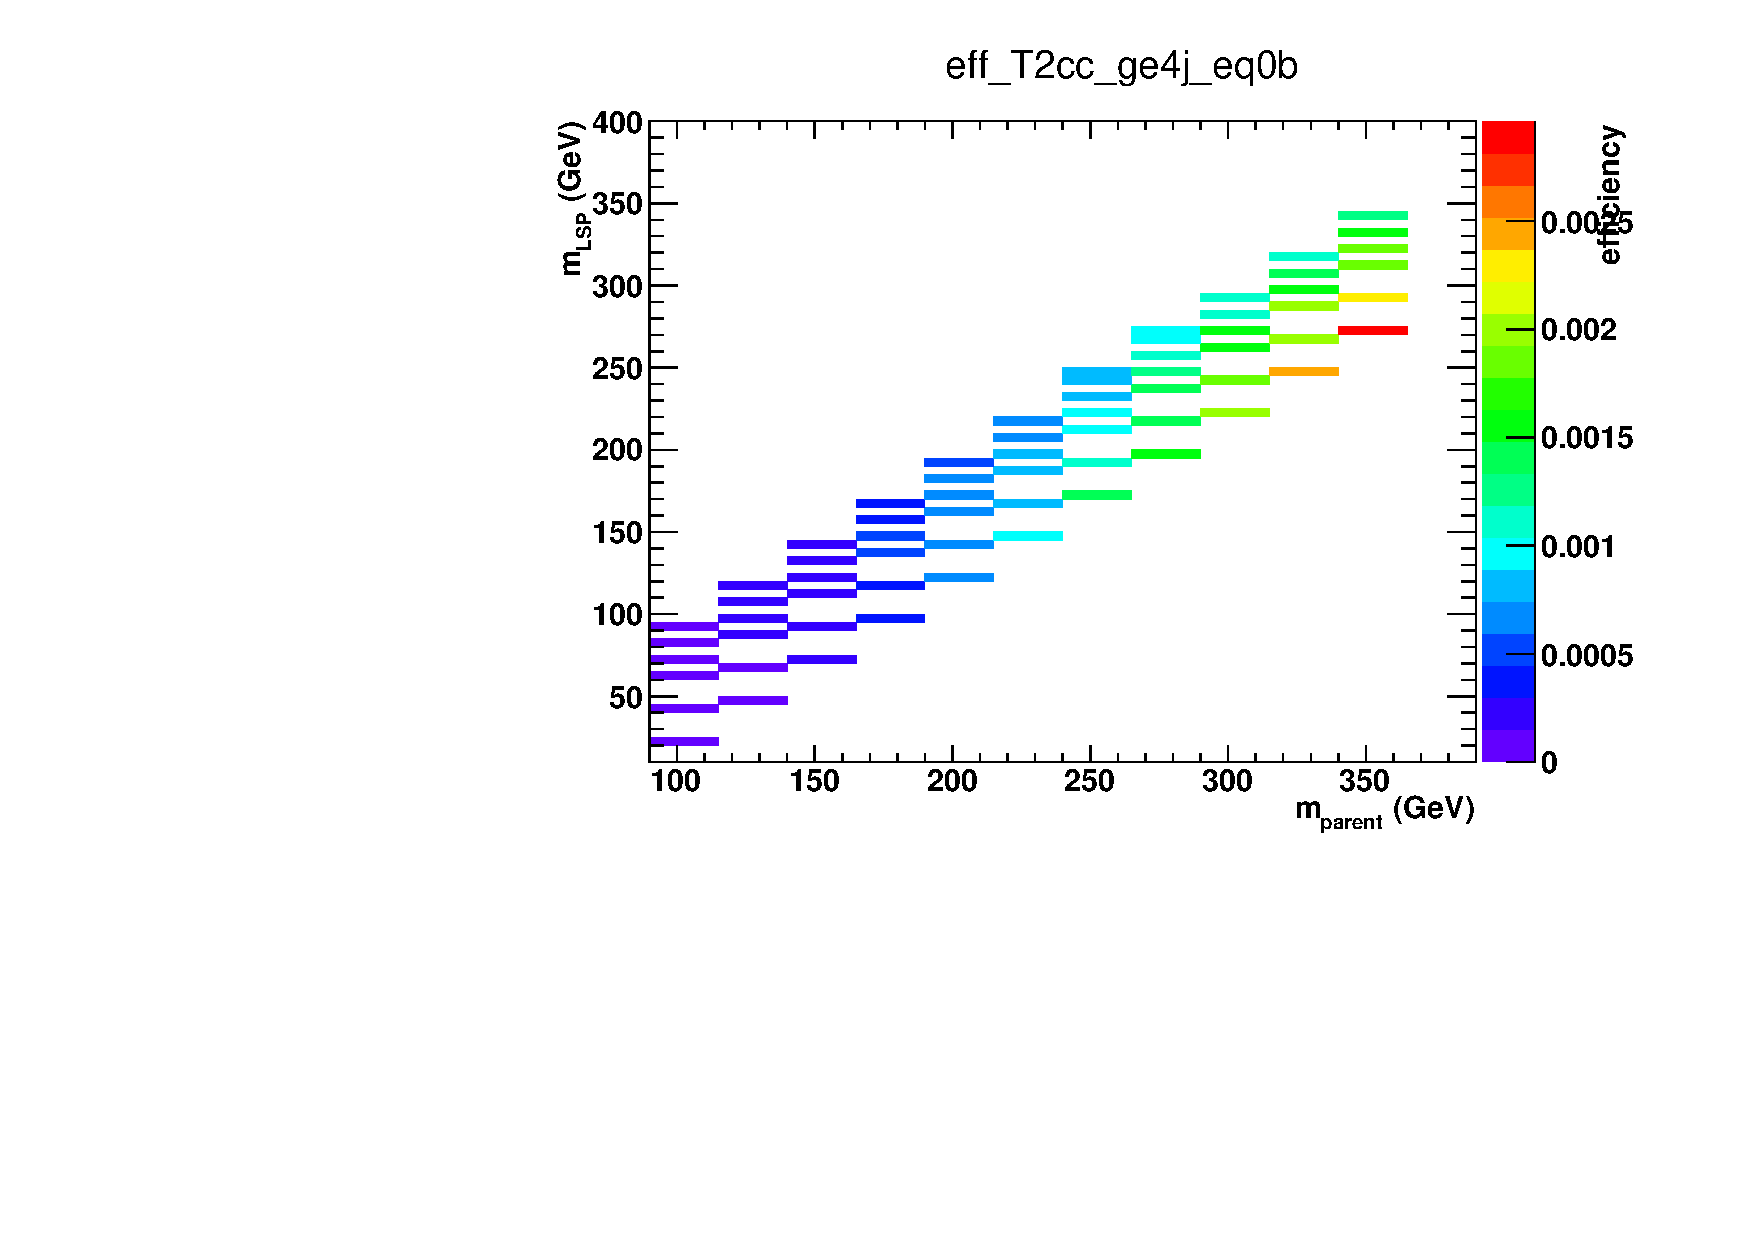
\includegraphics[width=0.4\textwidth,page=1]{figures/sms/t2cc/v1/T2cc_eff}
    } 
    \subfigure[Hadronic Selection Efficiency, ($\geq 4$,1)]{
      \includegraphics[width=0.4\textwidth,page=2]{figures/sms/t2cc/v1/T2cc_eff}
    } 
    \caption{Hadronic selection efficiency times acceptance for \texttt{T2cc}
      for the relevant event categories defined by \njet and \nb.
      Note the different z-axis scales.}
    \label{fig:sms-eff-t2cc}
  \end{center}
\end{figure}

%\begin{figure}[h!]
%  \begin{center}
%    \subfigure[$m_{\sTop} = 250\gev, m_{\rm LSP} = 170\gev$]{
%      \includegraphics[width=0.6\textwidth, trim=0 0 0 30, clip=true]{figures/sms/t2cc/v25/T2cc_sig_inj_250_170}
%    } \\
%%    \subfigure[$m_{\sTop} = 250\gev, m_{\rm LSP} = 230\gev$]{
%%      \includegraphics[width=0.6\textwidth, trim=0 0 0 30, clip=true]{figures/sms/t2cc/v25/T2cc_sig_inj_250_230}
%%    } \\
%    \subfigure[$m_{\sTop} = 250\gev, m_{\rm LSP} = 240\gev$]{
%      \includegraphics[width=0.6\textwidth, trim=0 0 0 30, clip=true]{figures/sms/t2cc/v25/T2cc_sig_inj_250_240}
%    } \\
%    \caption{The expected signal significance (in terms of the number
%      of standard deviations) per signal region bin for the
%      \texttt{T2cc} model with $m_{\sTop} = 250\gev$ and $m_{\rm LSP}
%      = 170\gev$ (Top) and $m_{\rm LSP} = 170\gev$ (Bottom).}
%    % the best fit point $m_{\rm LSP} = 170\gev$ (Middle) 
%    \label{fig:sms-t2cc-sig}
%  \end{center}
%\end{figure}

%\begin{figure}[h!]
%  \begin{center}
%    \subfigure[\label{fig:sms-pdf-up-t2cc}$+1\sigma$]{
%      \includegraphics[width=0.6\textwidth]{figures/sms/t2cc/acc_pSigmaRel_m0_m12}
%    }\\
%    \subfigure[\label{fig:sms-pdf-t2cc-nominal}Nominal]{
%      \includegraphics[width=0.6\textwidth]{figures/sms/t2cc/acc_cvRel_m0_m12}
%    }\\
%    \subfigure[\label{fig:sms-pdf-down-t2cc}$-1\sigma$]{
%      \includegraphics[width=0.6\textwidth]{figures/sms/t2cc/acc_mSigmaRel_m0_m12}
%    }\\  
%    \caption{\label{fig:sms-pdf-t2cc}Ratio of efficiency times
%      acceptance for the (middle) central value, (top) $+1\sigma$
%      value, (bottom) $-1\sigma$ value of the envelope calculation
%      relative to the nominal PDF set used to produce the
%      \texttt{T2cc} sample. }
%  \end{center}
%\end{figure}

\begin{figure}[h!]
  \begin{center}
    \subfigure[\njetlow, $\nb = 0$.]{
      \includegraphics[width=0.35\textwidth, page=4]{figures/sms/t2cc/v1/t2cc_unc}
    }
    \subfigure[\njetlow, $\nb = 0$.]{
      \includegraphics[width=0.35\textwidth, page=6]{figures/sms/t2cc/v1/t2cc_unc}
    }\\
    \subfigure[\njetlow, $\nb = 1$.]{
      \includegraphics[width=0.35\textwidth, page=4]{figures/sms/t2cc/v1/t2cc_unc}
    }
    \subfigure[\njetlow, $\nb = 1$.]{
      \includegraphics[width=0.35\textwidth, page=6]{figures/sms/t2cc/v1/t2cc_unc}
    }\\
    \subfigure[\njethigh, $\nb = 0$.]{
      \includegraphics[width=0.35\textwidth, page=4]{figures/sms/t2cc/v1/t2cc_unc}
    }
    \subfigure[\njethigh, $\nb = 0$.]{
      \includegraphics[width=0.35\textwidth, page=6]{figures/sms/t2cc/v1/t2cc_unc}
    }\\
    \subfigure[\njethigh, $\nb = 1$.]{
      \includegraphics[width=0.35\textwidth, page=4]{figures/sms/t2cc/v1/t2cc_unc}
    }  
    \subfigure[\njethigh, $\nb = 1$.]{
      \includegraphics[width=0.35\textwidth, page=6]{figures/sms/t2cc/v1/t2cc_unc}
    }\\
    \caption{\label{fig:sms-jes-t2cc}The fractional change in
      signal efficiency due to systematically (Left) increasing and
      (Middle) decreasing all jet energies, and (Right) the resulting
      (symmetric) systematic uncertainties due to JES uncertainties
      for \texttt{T2cc}.}
  \end{center}
\end{figure}

\begin{figure}[h!]
  \begin{center}
    \subfigure[\njetlow, $\nb = 0$.]{
      \includegraphics[width=0.35\textwidth, page=4]{figures/sms/t2cc/v1/t2cc_unc}
    }
    \subfigure[\njetlow, $\nb = 0$.]{
      \includegraphics[width=0.35\textwidth, page=6]{figures/sms/t2cc/v1/t2cc_unc}
    }\\
    \subfigure[\njetlow, $\nb = 1$.]{
      \includegraphics[width=0.35\textwidth, page=4]{figures/sms/t2cc/v1/t2cc_unc}
    }
    \subfigure[\njetlow, $\nb = 1$.]{
      \includegraphics[width=0.35\textwidth, page=6]{figures/sms/t2cc/v1/t2cc_unc}
    }\\
    \subfigure[\njethigh, $\nb = 0$.]{
      \includegraphics[width=0.35\textwidth, page=4]{figures/sms/t2cc/v1/t2cc_unc}
    }
    \subfigure[\njethigh, $\nb = 0$.]{
      \includegraphics[width=0.35\textwidth, page=6]{figures/sms/t2cc/v1/t2cc_unc}
    }\\
    \subfigure[\njethigh, $\nb = 1$.]{
      \includegraphics[width=0.35\textwidth, page=4]{figures/sms/t2cc/v1/t2cc_unc}
    }  
    \subfigure[\njethigh, $\nb = 1$.]{
      \includegraphics[width=0.35\textwidth, page=6]{figures/sms/t2cc/v1/t2cc_unc}
    }\\
    \caption{\label{fig:sms-isr-t2cc}The fractional change in signal
      efficiency due to systematically (Left) increasing and (Middle)
      decreasing event weights according to ISR uncertainties, and
      (Right) the resulting (symmetric) systematic uncertainties due
      to ISR uncertainties for \texttt{T2cc}.}
  \end{center}
\end{figure}

\begin{figure}[h!]
  \begin{center}
    \subfigure[\njetlow, $\nb = 0$.]{
      \includegraphics[width=0.35\textwidth, page=4]{figures/sms/t2cc/v1/t2cc_unc}
    }
    \subfigure[\njetlow, $\nb = 0$.]{
      \includegraphics[width=0.35\textwidth, page=6]{figures/sms/t2cc/v1/t2cc_unc}
    }\\
    \subfigure[\njetlow, $\nb = 1$.]{
      \includegraphics[width=0.35\textwidth, page=4]{figures/sms/t2cc/v1/t2cc_unc}
    }
    \subfigure[\njetlow, $\nb = 1$.]{
      \includegraphics[width=0.35\textwidth, page=6]{figures/sms/t2cc/v1/t2cc_unc}
    }\\
    \subfigure[\njethigh, $\nb = 0$.]{
      \includegraphics[width=0.35\textwidth, page=4]{figures/sms/t2cc/v1/t2cc_unc}
    }
    \subfigure[\njethigh, $\nb = 0$.]{
      \includegraphics[width=0.35\textwidth, page=6]{figures/sms/t2cc/v1/t2cc_unc}
    }\\
    \subfigure[\njethigh, $\nb = 1$.]{
      \includegraphics[width=0.35\textwidth, page=4]{figures/sms/t2cc/v1/t2cc_unc}
    }  
    \subfigure[\njethigh, $\nb = 1$.]{
      \includegraphics[width=0.35\textwidth, page=6]{figures/sms/t2cc/v1/t2cc_unc}
    }\\
    \caption{\label{fig:sms-btag-t2cc}The fractional change in signal
      efficiency due to systematically (Left) increasing and (Middle)
      decreasing all b-tag efficiencies according to the scale factor
      uncertainties, and (Right) the resulting (symmetric) systematic
      uncertainties due to b-tag scale factor uncertainties for
      \texttt{T2cc}.} 
  \end{center}
\end{figure}

\begin{figure}[h!]
  \begin{center}
    \subfigure[\njetlow, $\nb = 0$.]{
     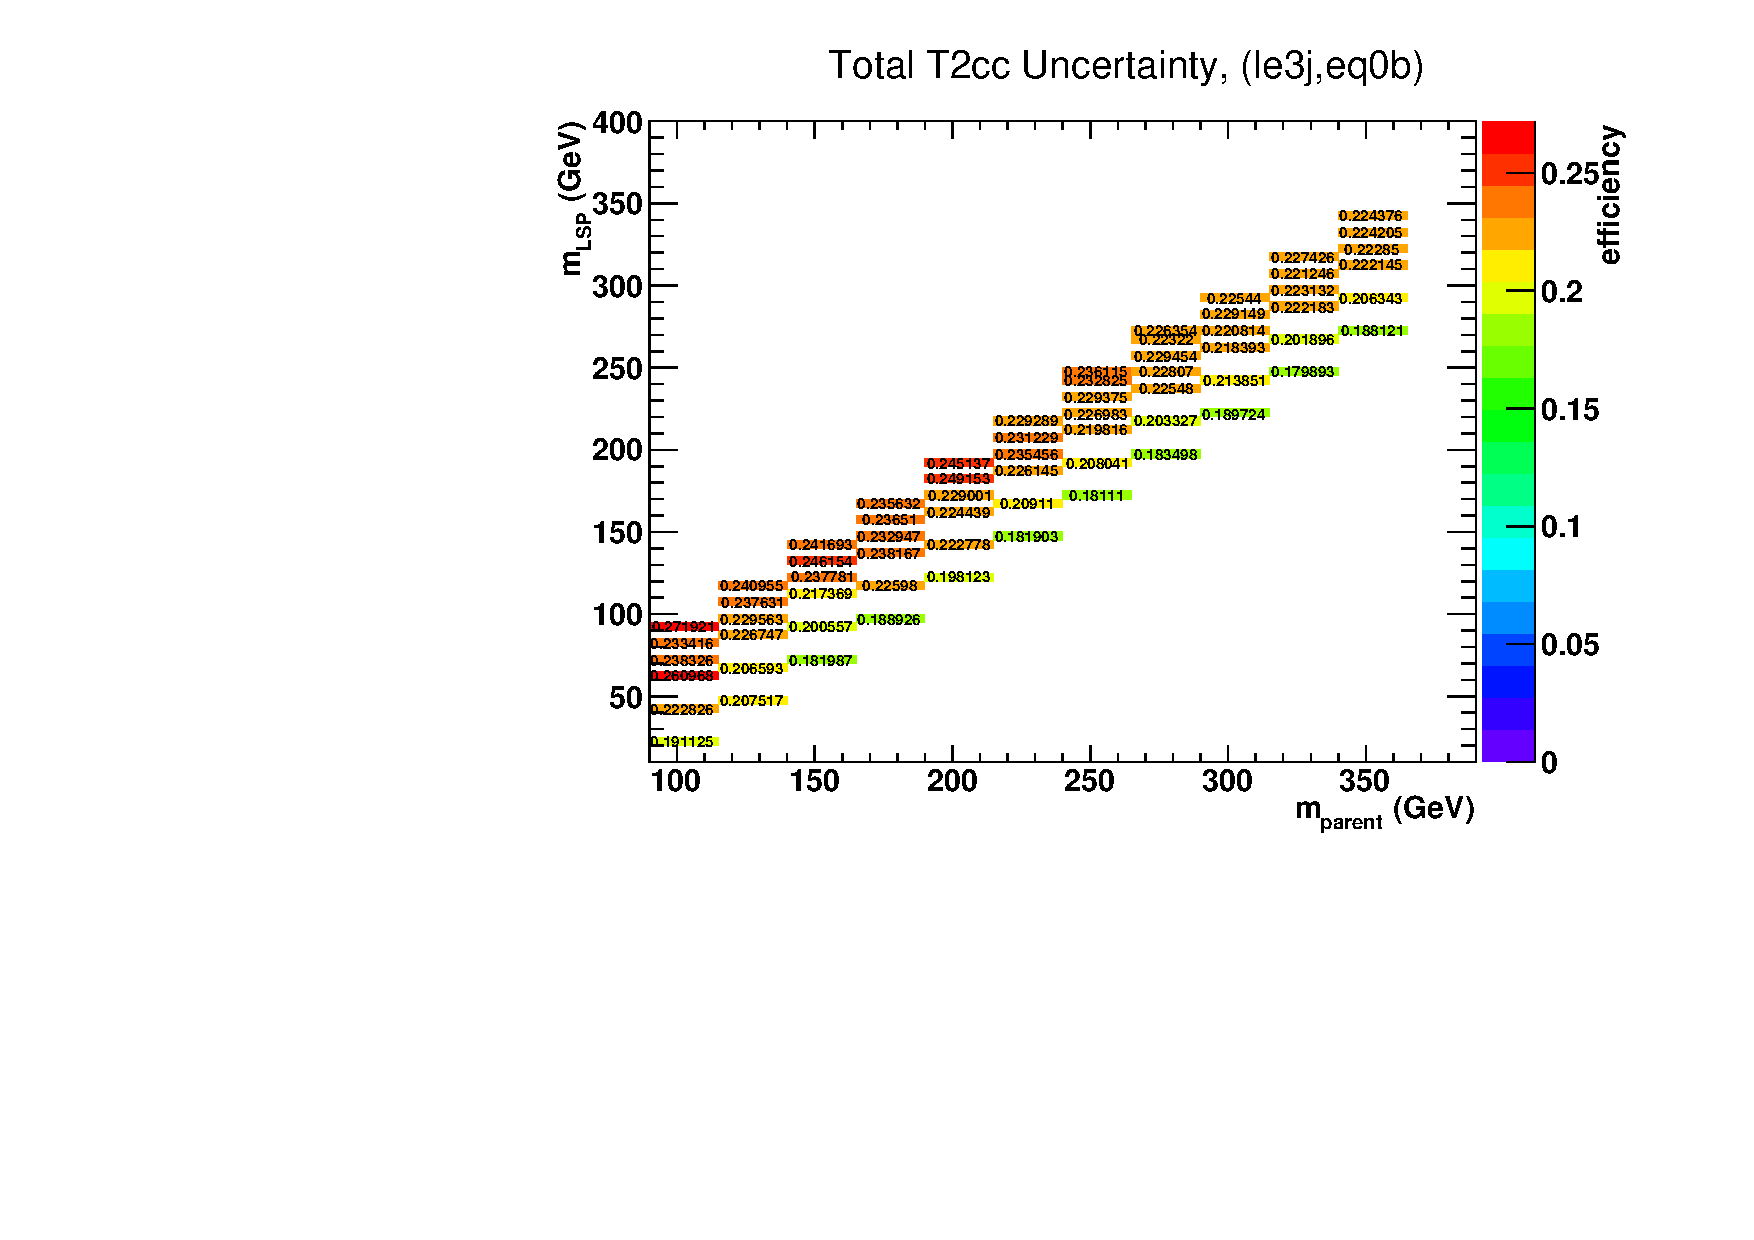
\includegraphics[width=0.48\textwidth,page=1]{figures/sms/t2cc/v1/t2cc_pfJet_totalUnc.pdf}
    }                                                                  
    \subfigure[\njetlow, $\nb = 1$.]{                                  
     \includegraphics[width=0.48\textwidth,page=2]{figures/sms/t2cc/v1/t2cc_pfJet_totalUnc.pdf}
    }\\                                                                
    \subfigure[\njethigh, $\nb = 0$.]{                                 
      \includegraphics[width=0.48\textwidth,page=5]{figures/sms/t2cc/v1/t2cc_pfJet_totalUnc.pdf}
    }                                                                  
    \subfigure[\njethigh, $\nb = 1$.]{                                 
      \includegraphics[width=0.48\textwidth,page=6]{figures/sms/t2cc/v1/t2cc_pfJet_totalUnc.pdf}
    }\\
    \caption{\label{fig:sms-total-t2cc}The total systematic
      uncertainty in the signal efficiency times acceptance for all
      relevant event categories for the \texttt{T2cc} intepretation.}
  \end{center}
\end{figure}

%%%%%%%%%%%%%%%%%%%%%%%%%%%%%%%%%%%%%%%%%%%%%%%%%%%%%%%%%%%%%%%%%%%%%%%%%%%%%%%%
%%%%%%%%%%%%%%%%%%%%%%%%%%%%%%%%%%%%%%%%%%%%%%%%%%%%%%%%%%%%%%%%%%%%%%%%%%%%%%%%
%%%%%%%%%%%%%%%%%%%%%%%%%%%%%%%%%%%%%%%%%%%%%%%%%%%%%%%%%%%%%%%%%%%%%%%%%%%%%%%%

%\clearpage
\subsection{T2tt\label{app:t2tt}}

\begin{figure}[h!]
  \begin{center}
    \subfigure[\njetlow, $\nb = 1$.]{
     \includegraphics[width=0.48\textwidth,page=2]{figures/sms/t2tt/v1/t2tt_pfJet_totalUnc.pdf}
    }
    \subfigure[\njetlow, $\nb = 2$.]{
     \includegraphics[width=0.48\textwidth,page=3]{figures/sms/t2tt/v1/t2tt_pfJet_totalUnc.pdf}
    }\\       
    \caption{\label{fig:sms-total-t2tt}The total systematic
      uncertainty in the signal efficiency times acceptance for all
      relevant event categories for the \texttt{T2tt} intepretation.}
  \end{center}
\end{figure}

%%%%%%%%%%%%%%%%%%%%%%%%%%%%%%%%%%%%%%%%%%%%%%%%%%%%%%%%%%%%%%%%%%%%%%%%%%%%%%%%
%%%%%%%%%%%%%%%%%%%%%%%%%%%%%%%%%%%%%%%%%%%%%%%%%%%%%%%%%%%%%%%%%%%%%%%%%%%%%%%%
%%%%%%%%%%%%%%%%%%%%%%%%%%%%%%%%%%%%%%%%%%%%%%%%%%%%%%%%%%%%%%%%%%%%%%%%%%%%%%%%

\clearpage
\subsection{T2tt\label{app:t2tt}}

\begin{figure}[!h]
  \begin{center}
    \subfigure[Hadronic Selection Efficiency, (2--3,1)]{
      \includegraphics[width=0.4\textwidth,page=7]{figures/sms/t2tt/v1/T2tt_eff}
    } 
    \subfigure[Hadronic Selection Efficiency, (2--3,2)]{
      \includegraphics[width=0.4\textwidth,page=8]{figures/sms/t2tt/v1/T2tt_eff}
    } \\
%    \subfigure[Hadronic Selection Efficiency, ($\geq 4$,0)]{
%      \includegraphics[width=0.4\textwidth]{figures/sms/t2_4body/v6/T2_4body_had_eff_maps_eq0b_ge4j_SITV}
%    }     
%    \subfigure[Hadronic Selection Efficiency, ($\geq 4$,1)]{
%      \includegraphics[width=0.4\textwidth]{figures/sms/t2_4body/v6/T2_4body_had_eff_maps_eq1b_ge4j_SITV}
%    } \\
    \caption{Hadronic selection efficiency times acceptance for the \texttt{T2tt}
      for the relevant event categories defined by \njet and \nb.
       Note the different z-axis scales.}
    \label{fig:sms-eff-t2_4body}
  \end{center}
\end{figure}

%\begin{figure}[h!]
%  \begin{center}
%    \subfigure[\njetlow, $\nb = 0$.]{
%      \includegraphics[width=0.35\textwidth, page=4]{figures/sms/t2_4body/v6/T2_4body_unc}
%    }
%    \subfigure[\njetlow, $\nb = 0$.]{
%      \includegraphics[width=0.35\textwidth, page=6]{figures/sms/t2_4body/v6/T2_4body_unc}
%    }
%    \subfigure[\njetlow, $\nb = 0$.]{
%      \includegraphics[width=0.35\textwidth, page=7]{figures/sms/t2_4body/v6/T2_4body_unc}
%    }\\
%    \subfigure[\njetlow, $\nb = 1$.]{
%      \includegraphics[width=0.35\textwidth, page=4]{figures/sms/t2_4body/v6/T2_4body_JES_eq1b_le3j}
%    }
%    \subfigure[\njetlow, $\nb = 1$.]{
%      \includegraphics[width=0.35\textwidth, page=6]{figures/sms/t2_4body/v6/T2_4body_JES_eq1b_le3j}
%    }
%    \subfigure[\njetlow, $\nb = 1$.]{
%      \includegraphics[width=0.35\textwidth, page=7]{figures/sms/t2_4body/v6/T2_4body_JES_eq1b_le3j}
%    }\\
%    \subfigure[\njethigh, $\nb = 0$.]{
%      \includegraphics[width=0.35\textwidth, page=4]{figures/sms/t2_4body/v6/T2_4body_JES_eq0b_ge4j}
%    }
%    \subfigure[\njethigh, $\nb = 0$.]{
%      \includegraphics[width=0.35\textwidth, page=6]{figures/sms/t2_4body/v6/T2_4body_JES_eq0b_ge4j}
%    }
%    \subfigure[\njethigh, $\nb = 0$.]{
%      \includegraphics[width=0.35\textwidth, page=7]{figures/sms/t2_4body/v6/T2_4body_JES_eq0b_ge4j}
%    }\\
%    \subfigure[\njethigh, $\nb = 1$.]{
%      \includegraphics[width=0.35\textwidth, page=4]{figures/sms/t2_4body/v6/T2_4body_JES_eq1b_ge4j}
%    }  
%    \subfigure[\njethigh, $\nb = 1$.]{
%      \includegraphics[width=0.35\textwidth, page=6]{figures/sms/t2_4body/v6/T2_4body_JES_eq1b_ge4j}
%    }
%    \subfigure[\njethigh, $\nb = 1$.]{
%      \includegraphics[width=0.35\textwidth, page=7]{figures/sms/t2_4body/v6/T2_4body_JES_eq1b_ge4j}
%    }\\
%    \caption{\label{fig:sms-jes-t2_4body}The fractional change in
%      signal efficiency due to systematically (Left) increasing and
%      (Middle) decreasing all jet energies, and (Right) the resulting
%      (symmetric) systematic uncertainties due to JES uncertainties
%      for \texttt{T2\_4body}.}
%  \end{center}
%\end{figure}
%
%\begin{figure}[h!]
%  \begin{center}
%    \subfigure[\njetlow, $\nb = 0$.]{
%      \includegraphics[width=0.35\textwidth, page=4]{figures/sms/t2_4body/v6/T2_4body_ISR_eq0b_le3j}
%    }
%    \subfigure[\njetlow, $\nb = 0$.]{
%      \includegraphics[width=0.35\textwidth, page=6]{figures/sms/t2_4body/v6/T2_4body_ISR_eq0b_le3j}
%    }
%    \subfigure[\njetlow, $\nb = 0$.]{
%      \includegraphics[width=0.35\textwidth, page=7]{figures/sms/t2_4body/v6/T2_4body_ISR_eq0b_le3j}
%    }\\
%    \subfigure[\njetlow, $\nb = 1$.]{
%      \includegraphics[width=0.35\textwidth, page=4]{figures/sms/t2_4body/v6/T2_4body_ISR_eq1b_le3j}
%    }
%    \subfigure[\njetlow, $\nb = 1$.]{
%      \includegraphics[width=0.35\textwidth, page=6]{figures/sms/t2_4body/v6/T2_4body_ISR_eq1b_le3j}
%    }
%    \subfigure[\njetlow, $\nb = 1$.]{
%      \includegraphics[width=0.35\textwidth, page=7]{figures/sms/t2_4body/v6/T2_4body_ISR_eq1b_le3j}
%    }\\
%    \subfigure[\njethigh, $\nb = 0$.]{
%      \includegraphics[width=0.35\textwidth, page=4]{figures/sms/t2_4body/v6/T2_4body_ISR_eq0b_ge4j}
%    }
%    \subfigure[\njethigh, $\nb = 0$.]{
%      \includegraphics[width=0.35\textwidth, page=6]{figures/sms/t2_4body/v6/T2_4body_ISR_eq0b_ge4j}
%    }
%    \subfigure[\njethigh, $\nb = 0$.]{
%      \includegraphics[width=0.35\textwidth, page=7]{figures/sms/t2_4body/v6/T2_4body_ISR_eq0b_ge4j}
%    }\\
%    \subfigure[\njethigh, $\nb = 1$.]{
%      \includegraphics[width=0.35\textwidth, page=4]{figures/sms/t2_4body/v6/T2_4body_ISR_eq1b_ge4j}
%    }  
%    \subfigure[\njethigh, $\nb = 1$.]{
%      \includegraphics[width=0.35\textwidth, page=6]{figures/sms/t2_4body/v6/T2_4body_ISR_eq1b_ge4j}
%    }
%    \subfigure[\njethigh, $\nb = 1$.]{
%      \includegraphics[width=0.35\textwidth, page=7]{figures/sms/t2_4body/v6/T2_4body_ISR_eq1b_ge4j}
%    }\\
%    \caption{\label{fig:sms-isr-t2_4body}The fractional change in signal
%      efficiency due to systematically (Left) increasing and (Middle)
%      decreasing event weights according to ISR uncertainties, and
%      (Right) the resulting (symmetric) systematic uncertainties due
%      to ISR uncertainties for \texttt{T2\_4body}.}
%  \end{center}
%\end{figure}
%
%\begin{figure}[h!]
%  \begin{center}
%    \subfigure[\njetlow, $\nb = 0$.]{
%      \includegraphics[width=0.35\textwidth, page=4]{figures/sms/t2_4body/v6/T2_4body_bTag_eq0b_le3j}
%    }
%    \subfigure[\njetlow, $\nb = 0$.]{
%      \includegraphics[width=0.35\textwidth, page=6]{figures/sms/t2_4body/v6/T2_4body_bTag_eq0b_le3j}
%    }
%    \subfigure[\njetlow, $\nb = 0$.]{
%      \includegraphics[width=0.35\textwidth, page=7]{figures/sms/t2_4body/v6/T2_4body_bTag_eq0b_le3j}
%    }\\
%    \subfigure[\njetlow, $\nb = 1$.]{
%      \includegraphics[width=0.35\textwidth, page=4]{figures/sms/t2_4body/v6/T2_4body_bTag_eq1b_le3j}
%    }
%    \subfigure[\njetlow, $\nb = 1$.]{
%      \includegraphics[width=0.35\textwidth, page=6]{figures/sms/t2_4body/v6/T2_4body_bTag_eq1b_le3j}
%    }
%    \subfigure[\njetlow, $\nb = 1$.]{
%      \includegraphics[width=0.35\textwidth, page=7]{figures/sms/t2_4body/v6/T2_4body_bTag_eq1b_le3j}
%    }\\
%    \subfigure[\njethigh, $\nb = 0$.]{
%      \includegraphics[width=0.35\textwidth, page=4]{figures/sms/t2_4body/v6/T2_4body_bTag_eq0b_ge4j}
%    }
%    \subfigure[\njethigh, $\nb = 0$.]{
%      \includegraphics[width=0.35\textwidth, page=6]{figures/sms/t2_4body/v6/T2_4body_bTag_eq0b_ge4j}
%    }
%    \subfigure[\njethigh, $\nb = 0$.]{
%      \includegraphics[width=0.35\textwidth, page=7]{figures/sms/t2_4body/v6/T2_4body_bTag_eq0b_ge4j}
%    }\\
%    \subfigure[\njethigh, $\nb = 1$.]{
%      \includegraphics[width=0.35\textwidth, page=4]{figures/sms/t2_4body/v6/T2_4body_bTag_eq1b_ge4j}
%    }  
%    \subfigure[\njethigh, $\nb = 1$.]{
%      \includegraphics[width=0.35\textwidth, page=6]{figures/sms/t2_4body/v6/T2_4body_bTag_eq1b_ge4j}
%    }
%    \subfigure[\njethigh, $\nb = 1$.]{
%      \includegraphics[width=0.35\textwidth, page=7]{figures/sms/t2_4body/v6/T2_4body_bTag_eq1b_ge4j}
%    }\\
%    \caption{\label{fig:sms-btag-t2_4body}The fractional change in signal
%      efficiency due to systematically (Left) increasing and (Middle)
%      decreasing all b-tag efficiencies according to the scale factor
%      uncertainties, and (Right) the resulting (symmetric) systematic
%      uncertainties due to b-tag scale factor uncertainties for
%      \texttt{T2\_4body}.} 
%  \end{center}
%\end{figure}
%
%\begin{figure}[h!]
% \begin{center}
%   \subfigure[\njetlow, $\nb = 0$.]{
%     \includegraphics[width=0.35\textwidth, page=4]{figures/sms/t2_4body/v6/T2_4body_MHT_MET_eq0b_le3j}
%   } \\
%   \subfigure[\njetlow, $\nb = 1$.]{
%     \includegraphics[width=0.35\textwidth, page=4]{figures/sms/t2_4body/v6/T2_4body_MHT_MET_eq1b_le3j}
%   } \\
%   \subfigure[\njethigh, $\nb = 0$.]{
%     \includegraphics[width=0.35\textwidth, page=4]{figures/sms/t2_4body/v6/T2_4body_MHT_MET_eq0b_ge4j}
%   } \\
%   \subfigure[\njethigh, $\nb = 1$.]{
%     \includegraphics[width=0.35\textwidth, page=4]{figures/sms/t2_4body/v6/T2_4body_MHT_MET_eq1b_ge4j}
%   } \\
%   \caption{\label{fig:sms-mht-met-t2_4body}The efficiency of the
%     $\mht/\met < 1.25$ requirement, for relative event categories. }
% \end{center}
%\end{figure}
%
%\begin{figure}[h!]
% \begin{center}
%   \subfigure[\njetlow, $\nb = 0$.]{
%     \includegraphics[width=0.35\textwidth, page=4]{figures/sms/t2_4body/v6/T2_4body_DeadECAL_eq0b_le3j}
%   } \\
%   \subfigure[\njetlow, $\nb = 1$.]{
%     \includegraphics[width=0.35\textwidth, page=4]{figures/sms/t2_4body/v6/T2_4body_DeadECAL_eq1b_le3j}
%   } \\
%   \subfigure[\njethigh, $\nb = 0$.]{
%     \includegraphics[width=0.35\textwidth, page=4]{figures/sms/t2_4body/v6/T2_4body_DeadECAL_eq0b_ge4j}
%   } \\
%   \subfigure[\njethigh, $\nb = 1$.]{
%     \includegraphics[width=0.35\textwidth, page=4]{figures/sms/t2_4body/v6/T2_4body_DeadECAL_eq1b_ge4j}
%   } \\
%   \caption{\label{fig:sms-dead-ecal-t2_4body}The efficiency of the dead
%     ECAL filter, for relative event categories. }
% \end{center}
%\end{figure}


\clearpage
\bibliography{alphaT}
\bibliographystyle{plain}


\end{document}   
